\chapter{Overall Description}
\label{chap:overall_description}%

\section{Product Perspective}
\label{sec:product_perspective}%

\subsection{Scenarios}
\label{sub:scenarios}%

\par{\textbf{Scenario 1: ST Login and CV Upload}} Walter W. is a chemical engineering student that wants to take part
in an internship to gain more experience and insight into the field before his graduation. Having heard of S\&C he
decides to give it a shot. First, he opens the S\&C website, where he clicks on the "Student Login" button. He is
prompted to enter his university-provided email and — after that — the platform redirects him to the SSO portal of this
institution (e.g., OpenID/OAuth…) where Walter can grant S\&C the permission to retrieve his information
(name, surname, birthdate, …) directly from his school. As soon as he grants our platform the required privileges, the
user is redirected to S\&C and his profile is created successfully. Now Walter has joined S\&C successfully, but he needs
to upload his CV; to do so he goes to the "My Profile" section where he can find the "My CV" subsection. Here, the user
can load his CV by uploading a PDF — preferably in a standard format (e.g., Europass, …) — version of it. Once uploaded,
the CV is indexed, and Walter can see a bullet list of possible improvements that he can make. The user is free to fix
his CV and re-upload an updated version iteratively once he is satisfied.

\par{\textbf{Scenario 2: ST Recruitment}} Saul G. is a freshly graduated law student, before starting his doctorate
he wants to gain some work experience before his research project starts. He joined S\&C but never found anything of his
linking; one day he receives an email from our platform regarding a possible internship: it is a law firm B.C.S. S.p.A.
looking for some intern to offload some work. Saul clicks on the link in the email and sees the internship details;
interested, the user clicks on "Apply." Some days later, Saul receives another email: it is S\&C informing him that the
company is interested in his profile and wants him to compile a survey to know him better. The user clicks on the link
and fills out the requested form. A week later, Saul receives a phone call from a lawyer, Kim, informing him that they
will work together: HR has found Saul as the idea candidate for the internship. During all the time of the selection
the user could see the internship status (when he has applied, if there are some forms to submit, …) from the
"My Internship" section so that no information is lost in case of accidental email deletion. Unread messages from S\&C
to the user can be seen on the "My Notification" section. Saul does his job very well and they are so impressed by his
work that they even offer him a full-time position in the company. At the "natural" end of the internship both STs and
COs are required to submit a final feedback describing how the experience was for both the parties involved.

\par{\textbf{Scenario 3: ST Sends a Feedback on the Internship}} Marie S. is an intern at a pharmaceutical company,
and she is starting to feel mistreated in her workplace: her boss yells at her for no reason all the time and she is
forced to do work outside what she agreed on. Marie goes to S\&C, finds her internship in the "My Internship" section
and clicks on "Submit feedback" and describes the situation. The next day, Marie receives a phone call from her
university: the internship is canceled, and appropriate actions will be taken against the corporation. The change in
the internship status is also visible in S\&C.

\par{\textbf{Scenario 4: CO Registration}} Tim I. is the CEO of a telecom company, TLC S.p.A. Having heard the
complaints from his VP of HR regarding the urgency of new workers, decides to enroll his company to S\&C hoping to find
skillful interns to then hire into the workforce. After a negotiation with the platform sales department, they agreed
to a fair contract between the parties. Then, a set of credentials is created to be used by an HR referent
– Tyrell W. — in TCL S.p.A.

\par{\textbf{Scenario 5: CO Publishes an Internship}} Tyrell W. — the HR referent for S\&C in TCL S.p.A. — log onto the
platform, using the "Company login" button, for the first time with the provided credentials. He is asked to build the
company’s profile on the platform by providing all necessary information (e.g., logo, mission, …); this profile will be
seen by the students that clicks on the company name on the various internship’s ads. The user now can go to the
"My Internship" section where he can create a new job posting; after all necessary information is provided the listing
is scanned and indexed. The company can see some suggestions on how to improve the ads copy: Tyrell is free to
iteratively adjust the ads until he is satisfied with the result.

\par{\textbf{Scenario 6: CO Recruitment}} After the registration deadline – having lots of applicants - Tyrell decides
to ask the students to fill out a questionnaire. He could have chosen to send it to a specific subset of applicants
– therefore rejecting students in the first phase of the recruitment process - but he decided to submit it to all of
them. S\&C automatically evaluates the response given by the students using the criteria provided by the company. After
the submission deadline Tyrell looks at the top 20 CV – ranked by the points gained in the questionnaire – and choose
the ten students to hire rejecting the unfit candidates. If Tyrell wanted, S\&C had recommended him directly some CVs
of students that were considered a good fit for the internship. These curricula were available in the "My Internship"
section and were properly anonymized to prevent any kind of bias. Tyrell, if he wanted, could have asked these students
to apply for the internship therefore increasing the number of total applicants. S\&C would have taken care of
notifying the students of the company's interest but the final decision on applying was left to the students.

\par{\textbf{Scenario 7: CO Sends a Feedback on the Internship}} During the internship, the students were tasked with
creating the engine that – given an address – returns the services TLC can offer at that location. The students,
however, failed in doing such: the tool-built returns lots of covered locations as unreachable by TCL network causing
serious economic damage for the company. Tyrell decides to go the "My Internship" section and send feedback to the
university. The next day the university calls TLC: the internship is suspended and the students fired.

\par{\textbf{Scenario 8: UN Registration}} PoliPo – Polytechnic University of Pordenone – is a well-known Italian
university. Their rector has decided that they are going to join S\&C to allow their students to gain some work
experience and to boost the "student employability" ranking of the university. After a negotiation with the platform
sales department, they agreed to a fair contract between the parties. The IT team of the university sent the details of
the authentication gateway to S\&C dev team: the platform now allows students and pre-designed university personnel to
login using the organization credentials.

\par{\textbf{Scenario 9: UN Deals with a Feedback}} Luca S., the project referent for S\&C in the school log onto the
platform using his PoliPo credentials. In the "My Internship" section he can see all ongoing and past internships
concerning only his students. In the "My Feedback" section he can see all the opened feedback by companies and
students. In this section he can reply to the message creator to further discuss the situation; a link here redirects
Luca on the proper internship in the "My Internship" section where he can suspend the internship.
Moreover, if necessary, Luca can prevent his students from seeing and applying for internship from a specific company
if he feels that these enterprises are mistreating his students. All blocked companies and the contracts between S\&C
and the university are available in the "My Contracts" section.

\subsection{Class Diagram}
\label{sub:class_diagram}%

\begin{figure}[H]
      \centering
      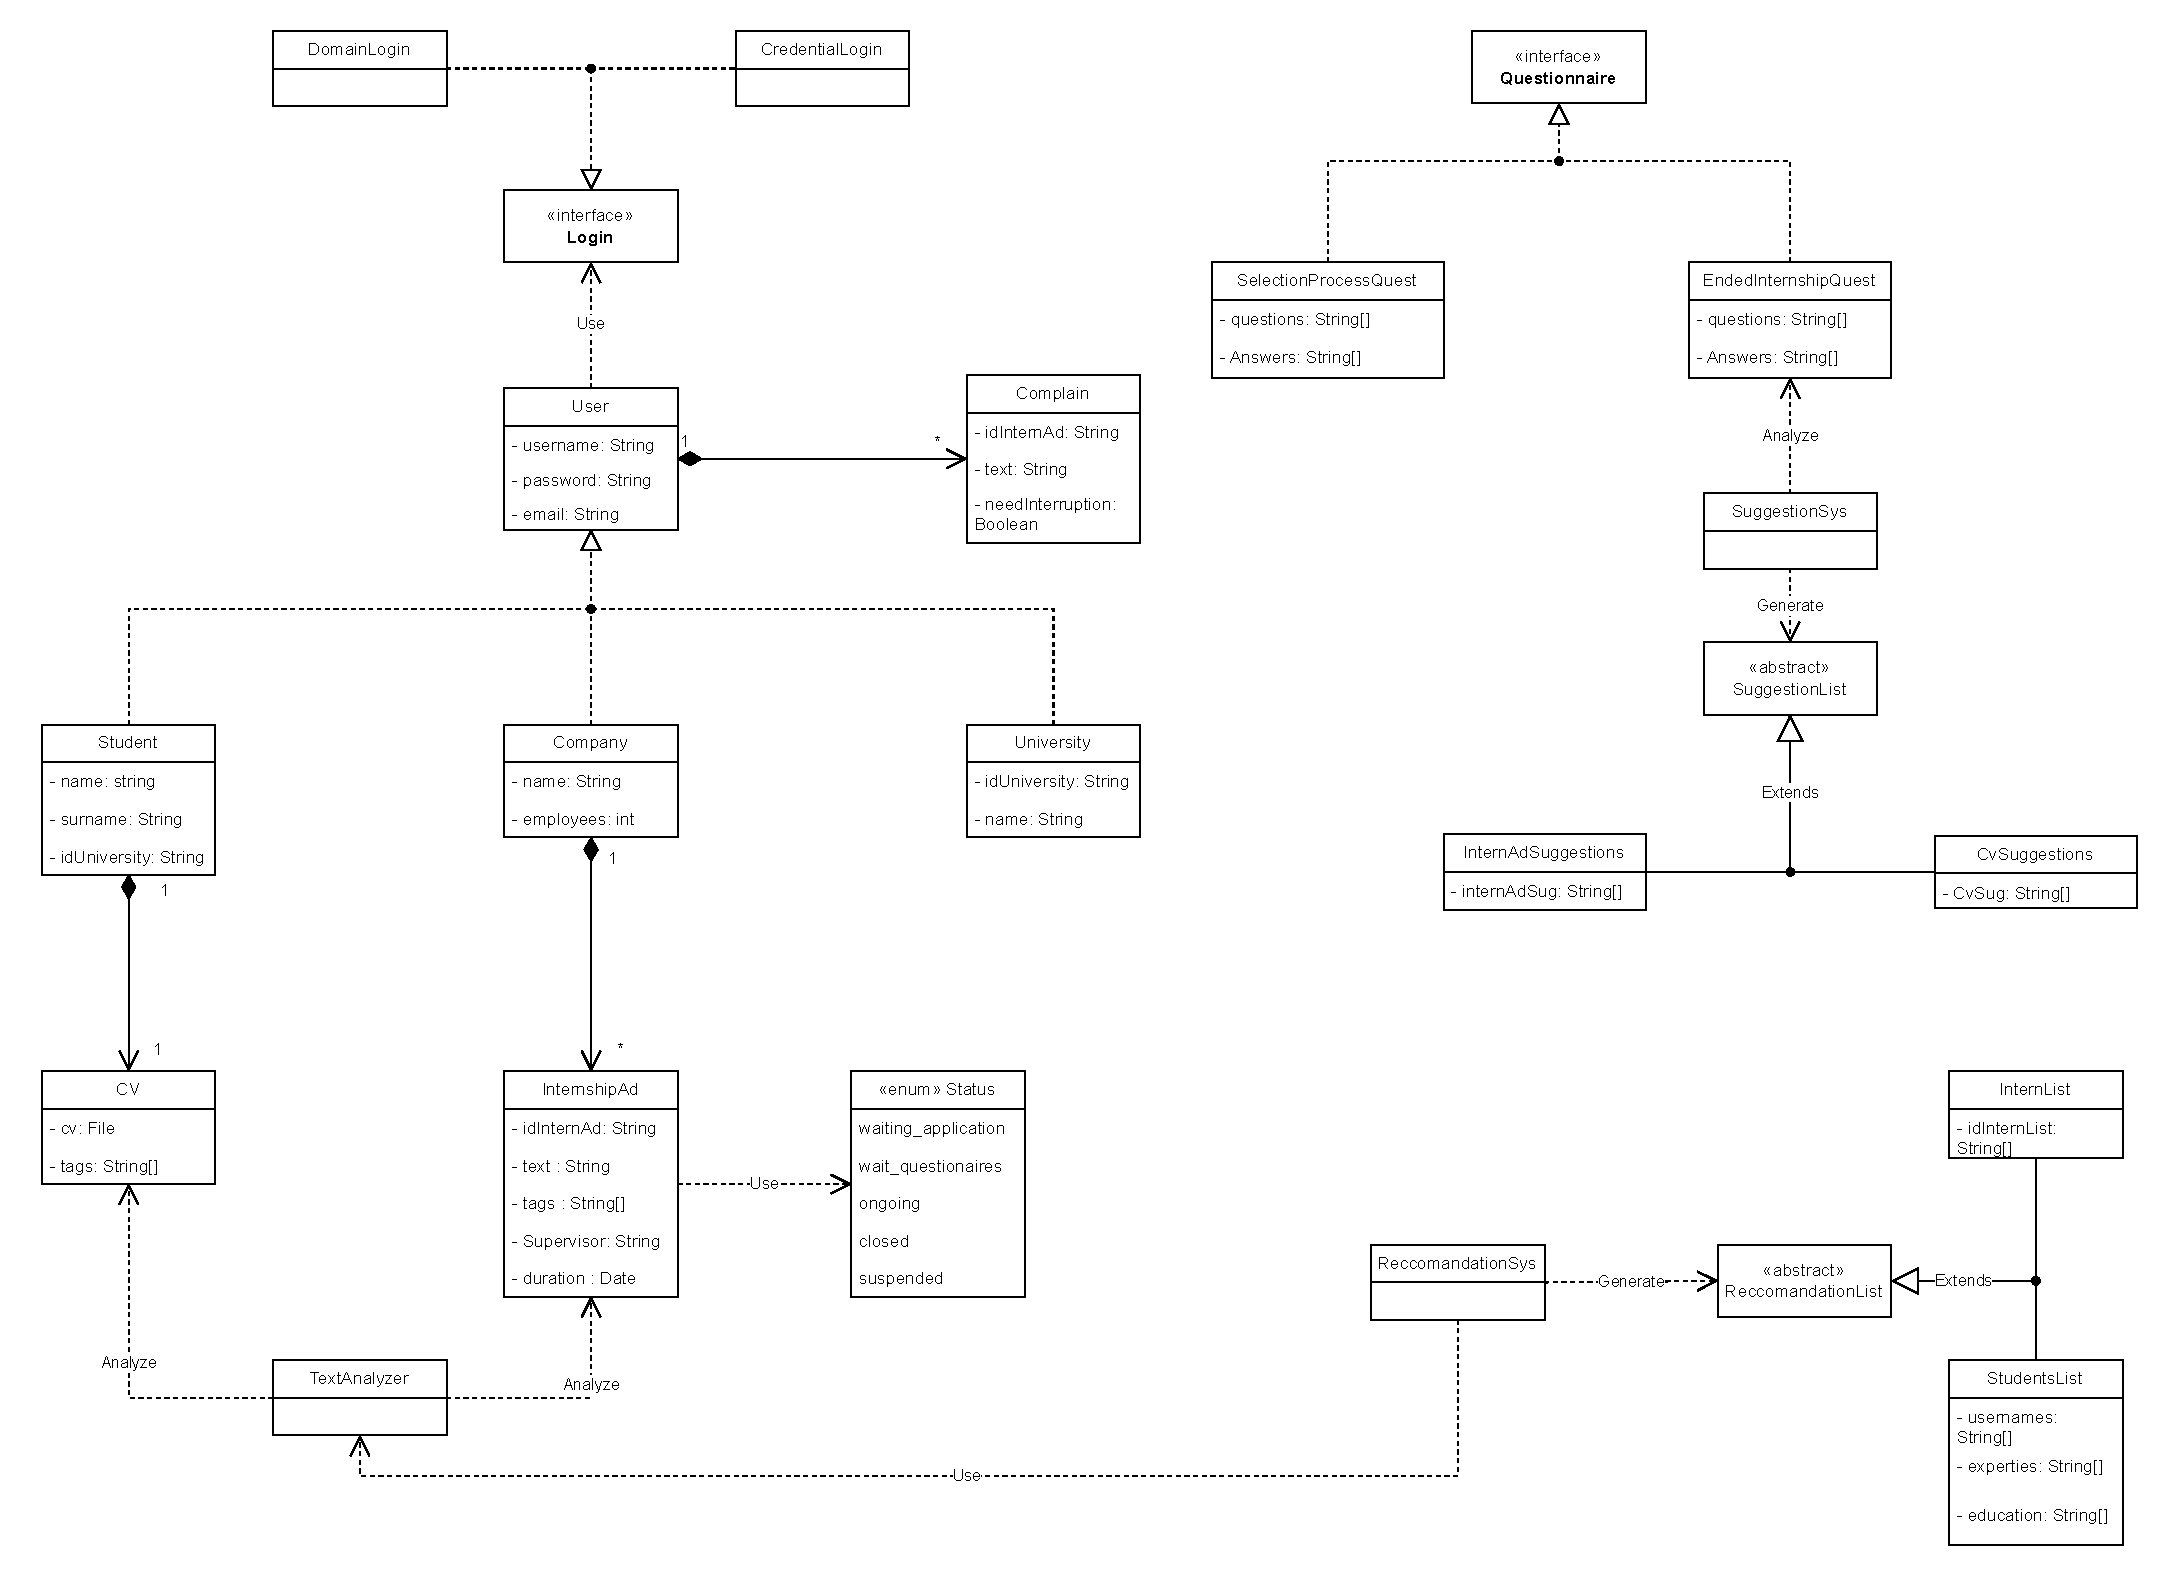
\includegraphics[width=1.0\textwidth]{Images/UML.pdf}
      \caption{High Level Class Diagram}
      \label{fig:class_diagram}
\end{figure}

\par The class diagram in figure \ref{fig:class_diagram} shows the high-level structure of the system. The classes of
the system actors, that are Student, Company, and University, are an extension of the User class, which is the base
class for all the users of the system, because all of them share some common attributes, the only difference is that
the password for the students is not set because they do the login through the university SSO.

\par The Student can upload a CV, that is stored in the system. The company can create an internship called
InternshipAd, which is stored in the system with a specific ID. The University can access all the internships and the
feedback of all the students that have it's university id.

\par Another important class is the questionnaire, which is an abstract class that is then extended into the selection
process questionnaire and feedback questionnaire, which are the two types of questionnaires that the system manages.
The first one is created by a CO to select the students for the internship, the second one is created by the system at
the end of the internship to collect feedback from both the student and the company. In this diagram are also
represented the subsystems that will do the analysis of the CVs and the internship ads, to create suggestions to
improve the CVs and the internship ads, and the one that is responsible for the recommendation that the students and
the companies receive by email.

\section{Product Functions}
\label{sec:product_functions}%

\par The following section describes the main functions of the system. The system is divided into three main actors:
the Student, the Company, and the University. Each of them has different functions that they can perform on the system.

\par\textbf{Generic Functionalities}

\begin{itemize}
      % F. 1
      \item \textbf{Account creation with verification}:
            We think that given the context in which S\&C will work there are ways improve on the creation of the
            accounts compared to the standard username, mail and password registration. Our idea is that S\&C will sell
            to both universities and companies the possibility of using the application and creating the accounts
            internally based on sales. For universities, when one university buys the S\&C service it will link its
            Active Directory to the S\&C database. This allows the student to access to S\&C with the university
            credentials. For companies, the account creation is handled internally, and the credentials are given to
            them after the contract is signed. With this mechanism we aim to make the platform more attractive for both
            parties because of the extra guarantees, in terms of verified users, that the account creation holds.

            \begin{figure}[H]
                  \centering
                  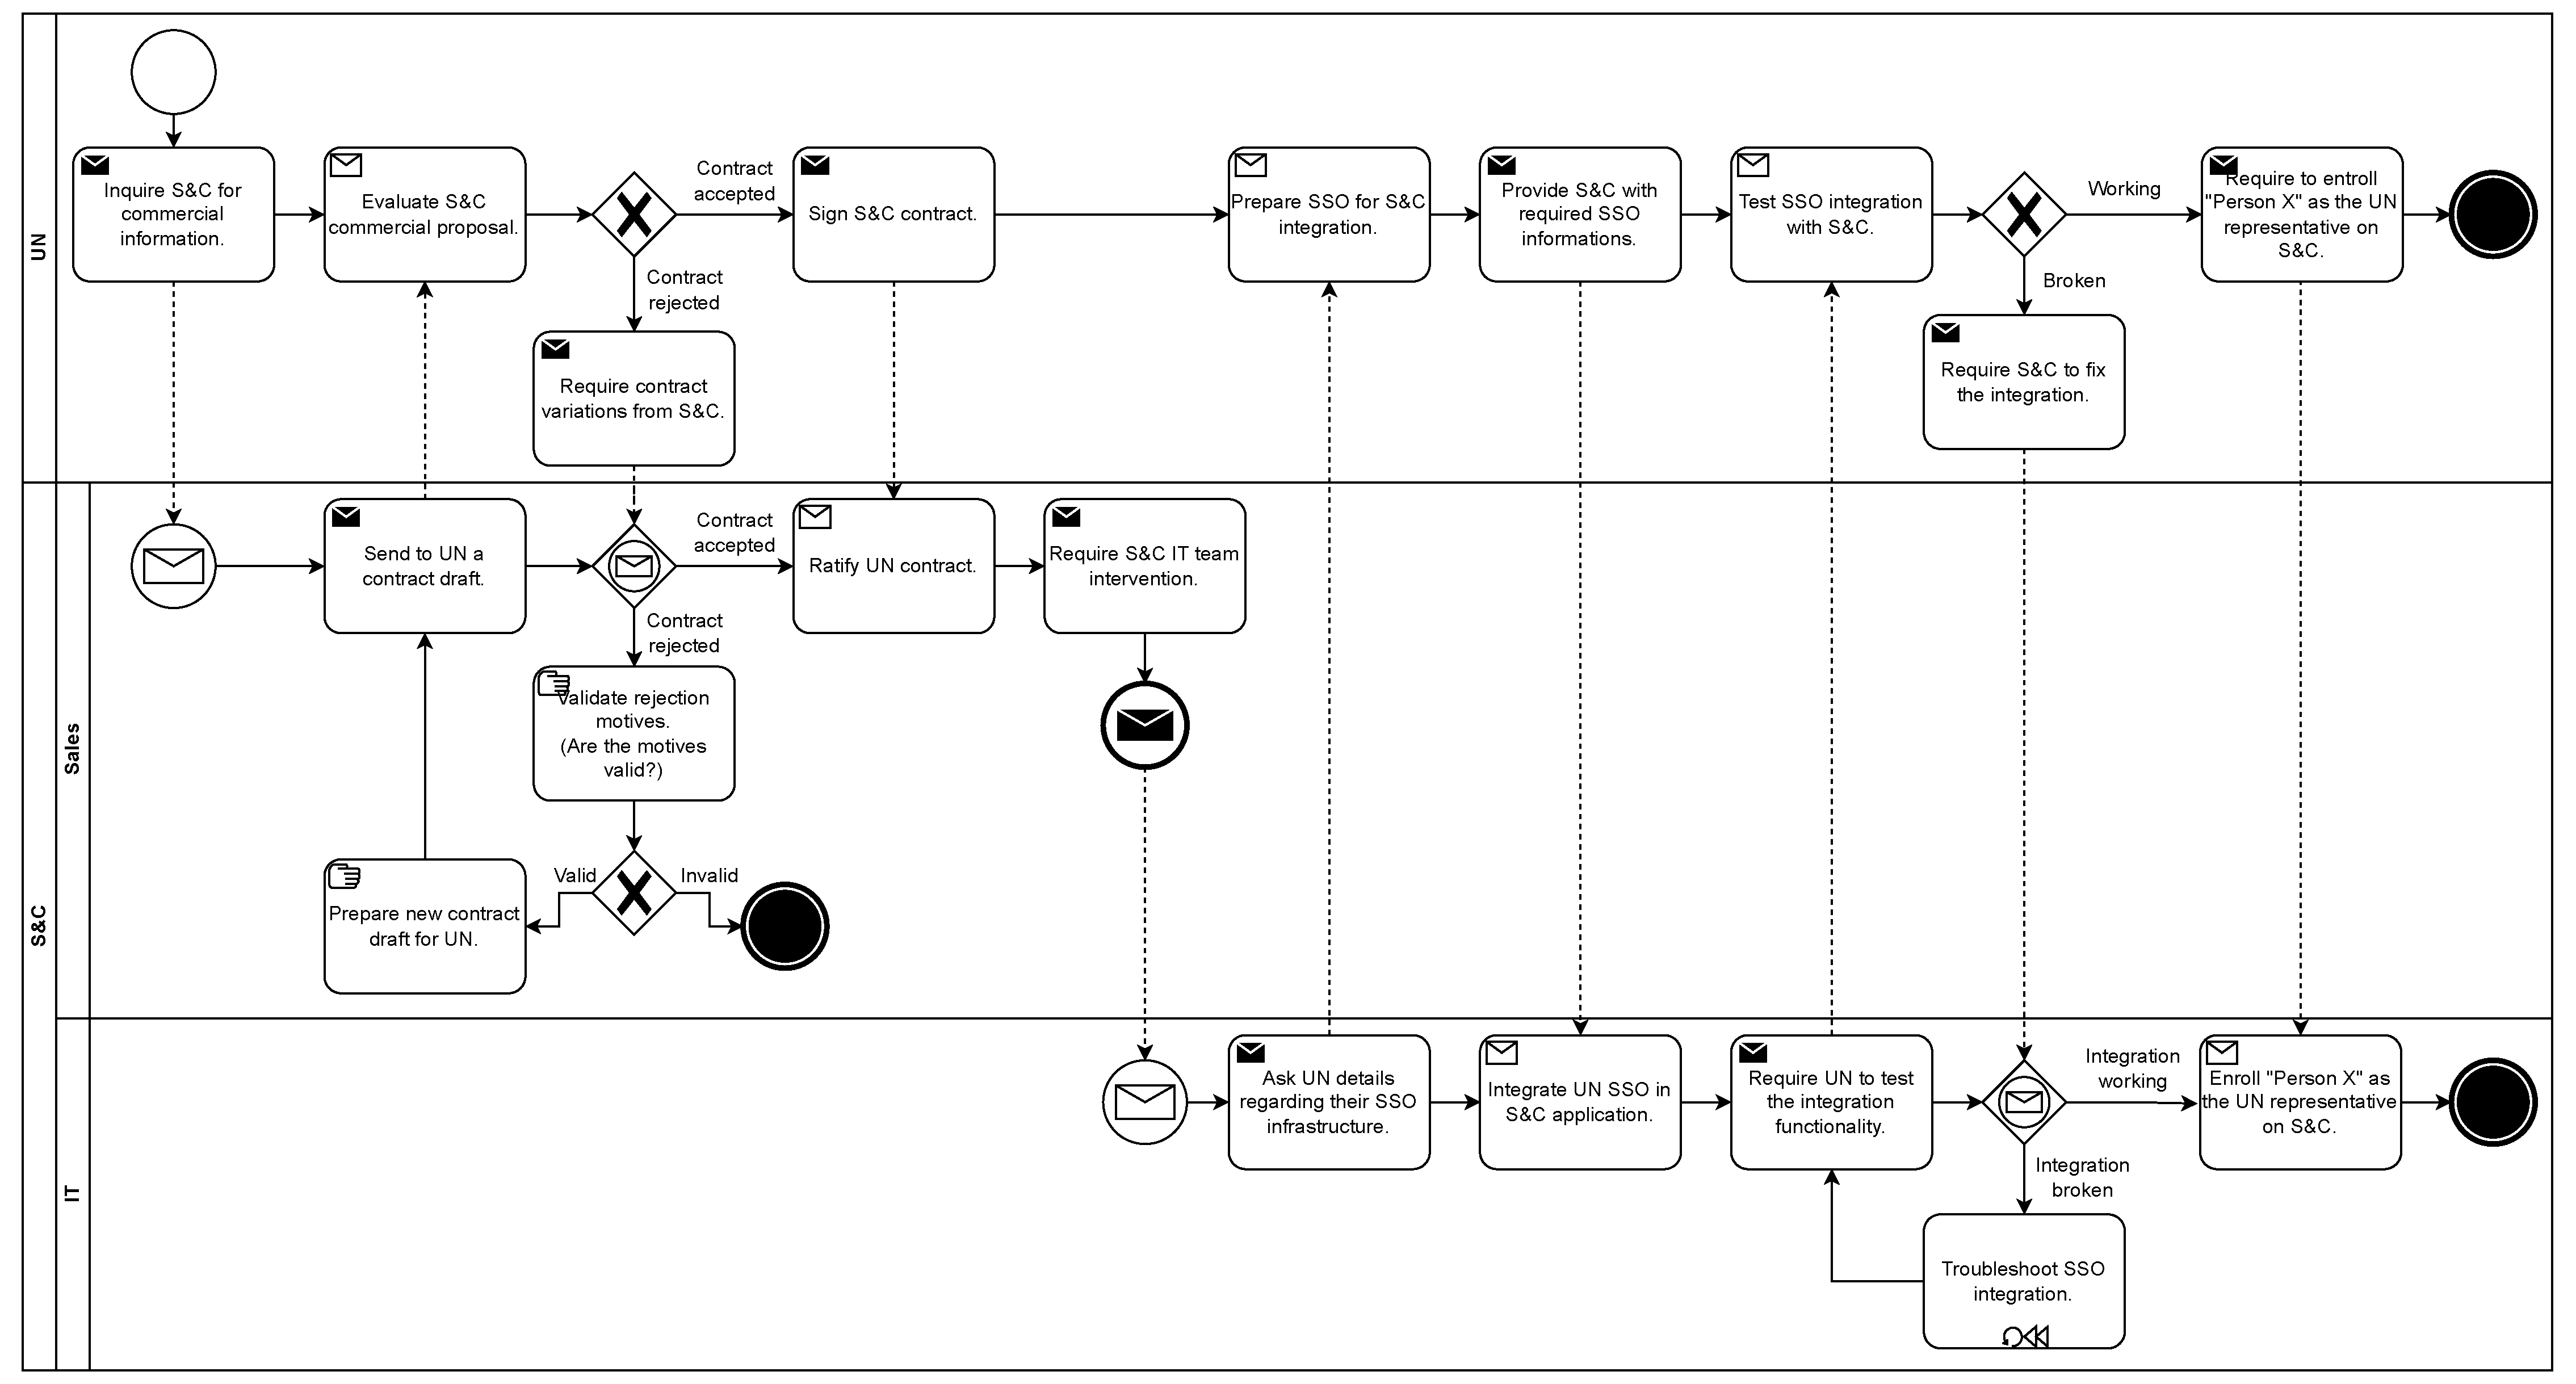
\includegraphics[width=1.0\textwidth]{Images/BPMN_1C.pdf}
                  \caption{UN Enrollment Diagram}
                  \label{fig:un_enrollment_diagram}
            \end{figure}

            \begin{figure}[H]
                  \centering
                  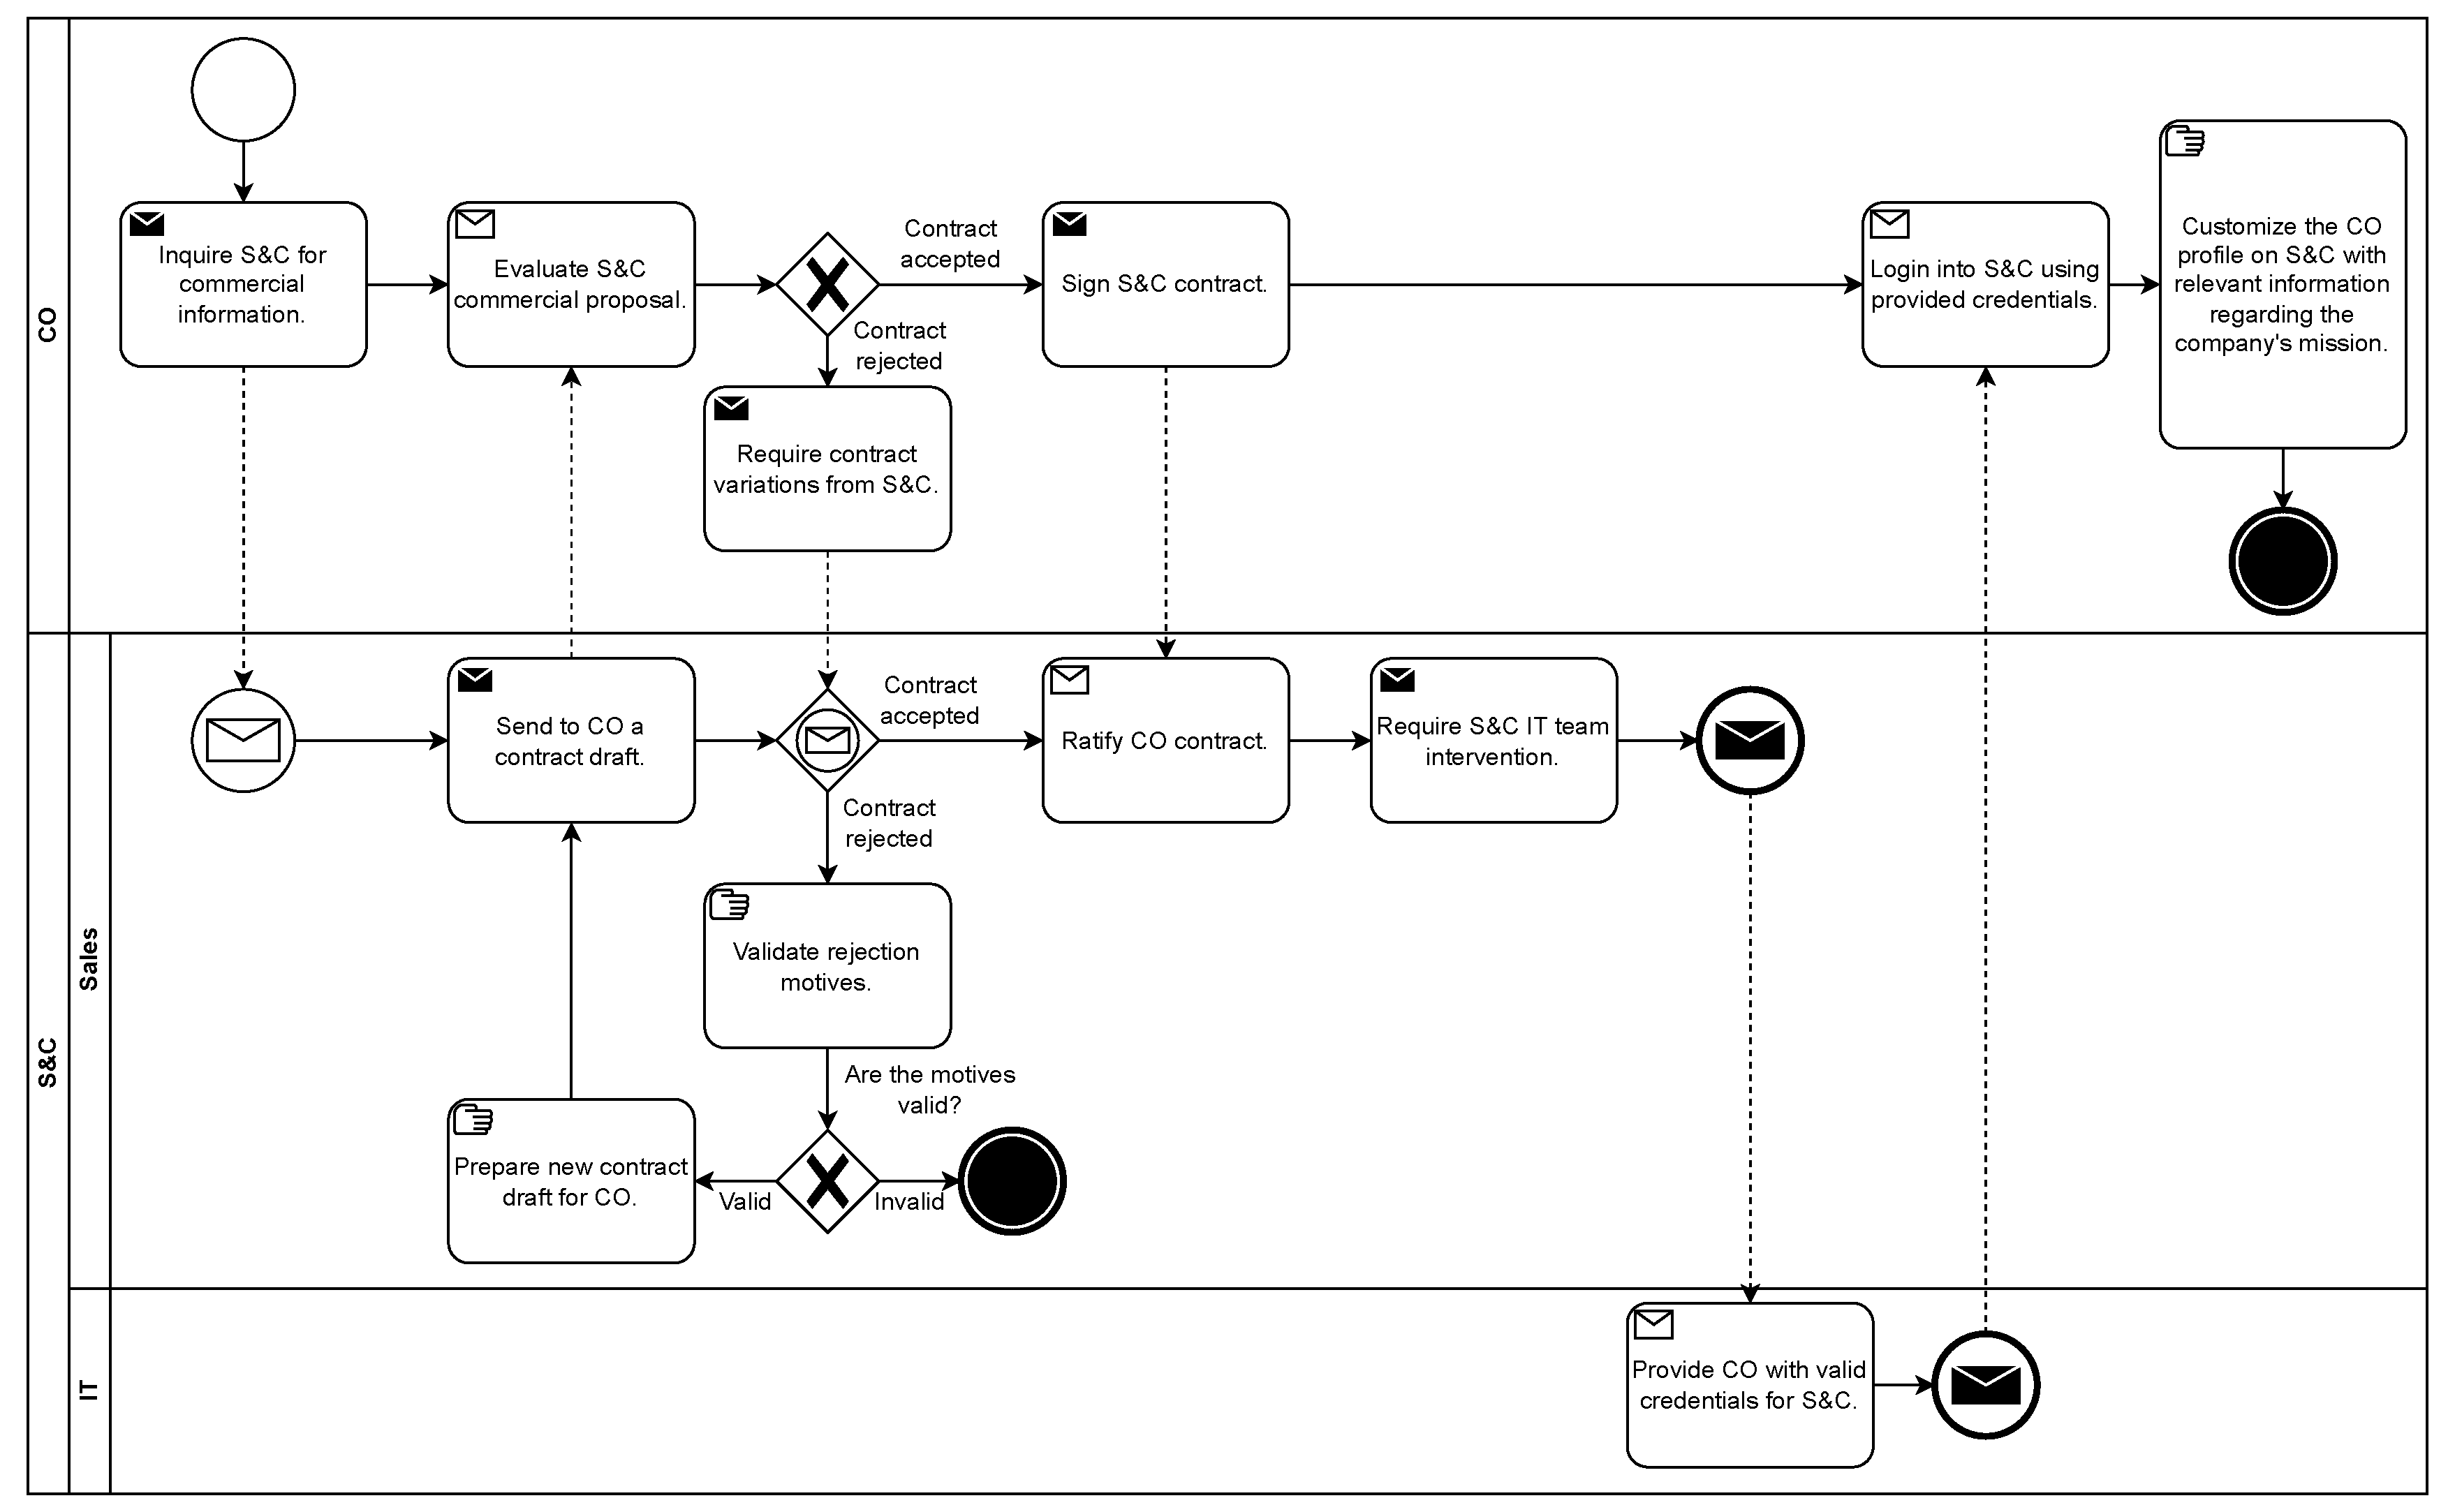
\includegraphics[width=1.0\textwidth]{Images/BPMN_1B.pdf}
                  \caption{CO Enrollment Diagram}
                  \label{fig:co_enrollment_diagram}
            \end{figure}

            \begin{figure}[H]
                  \centering
                  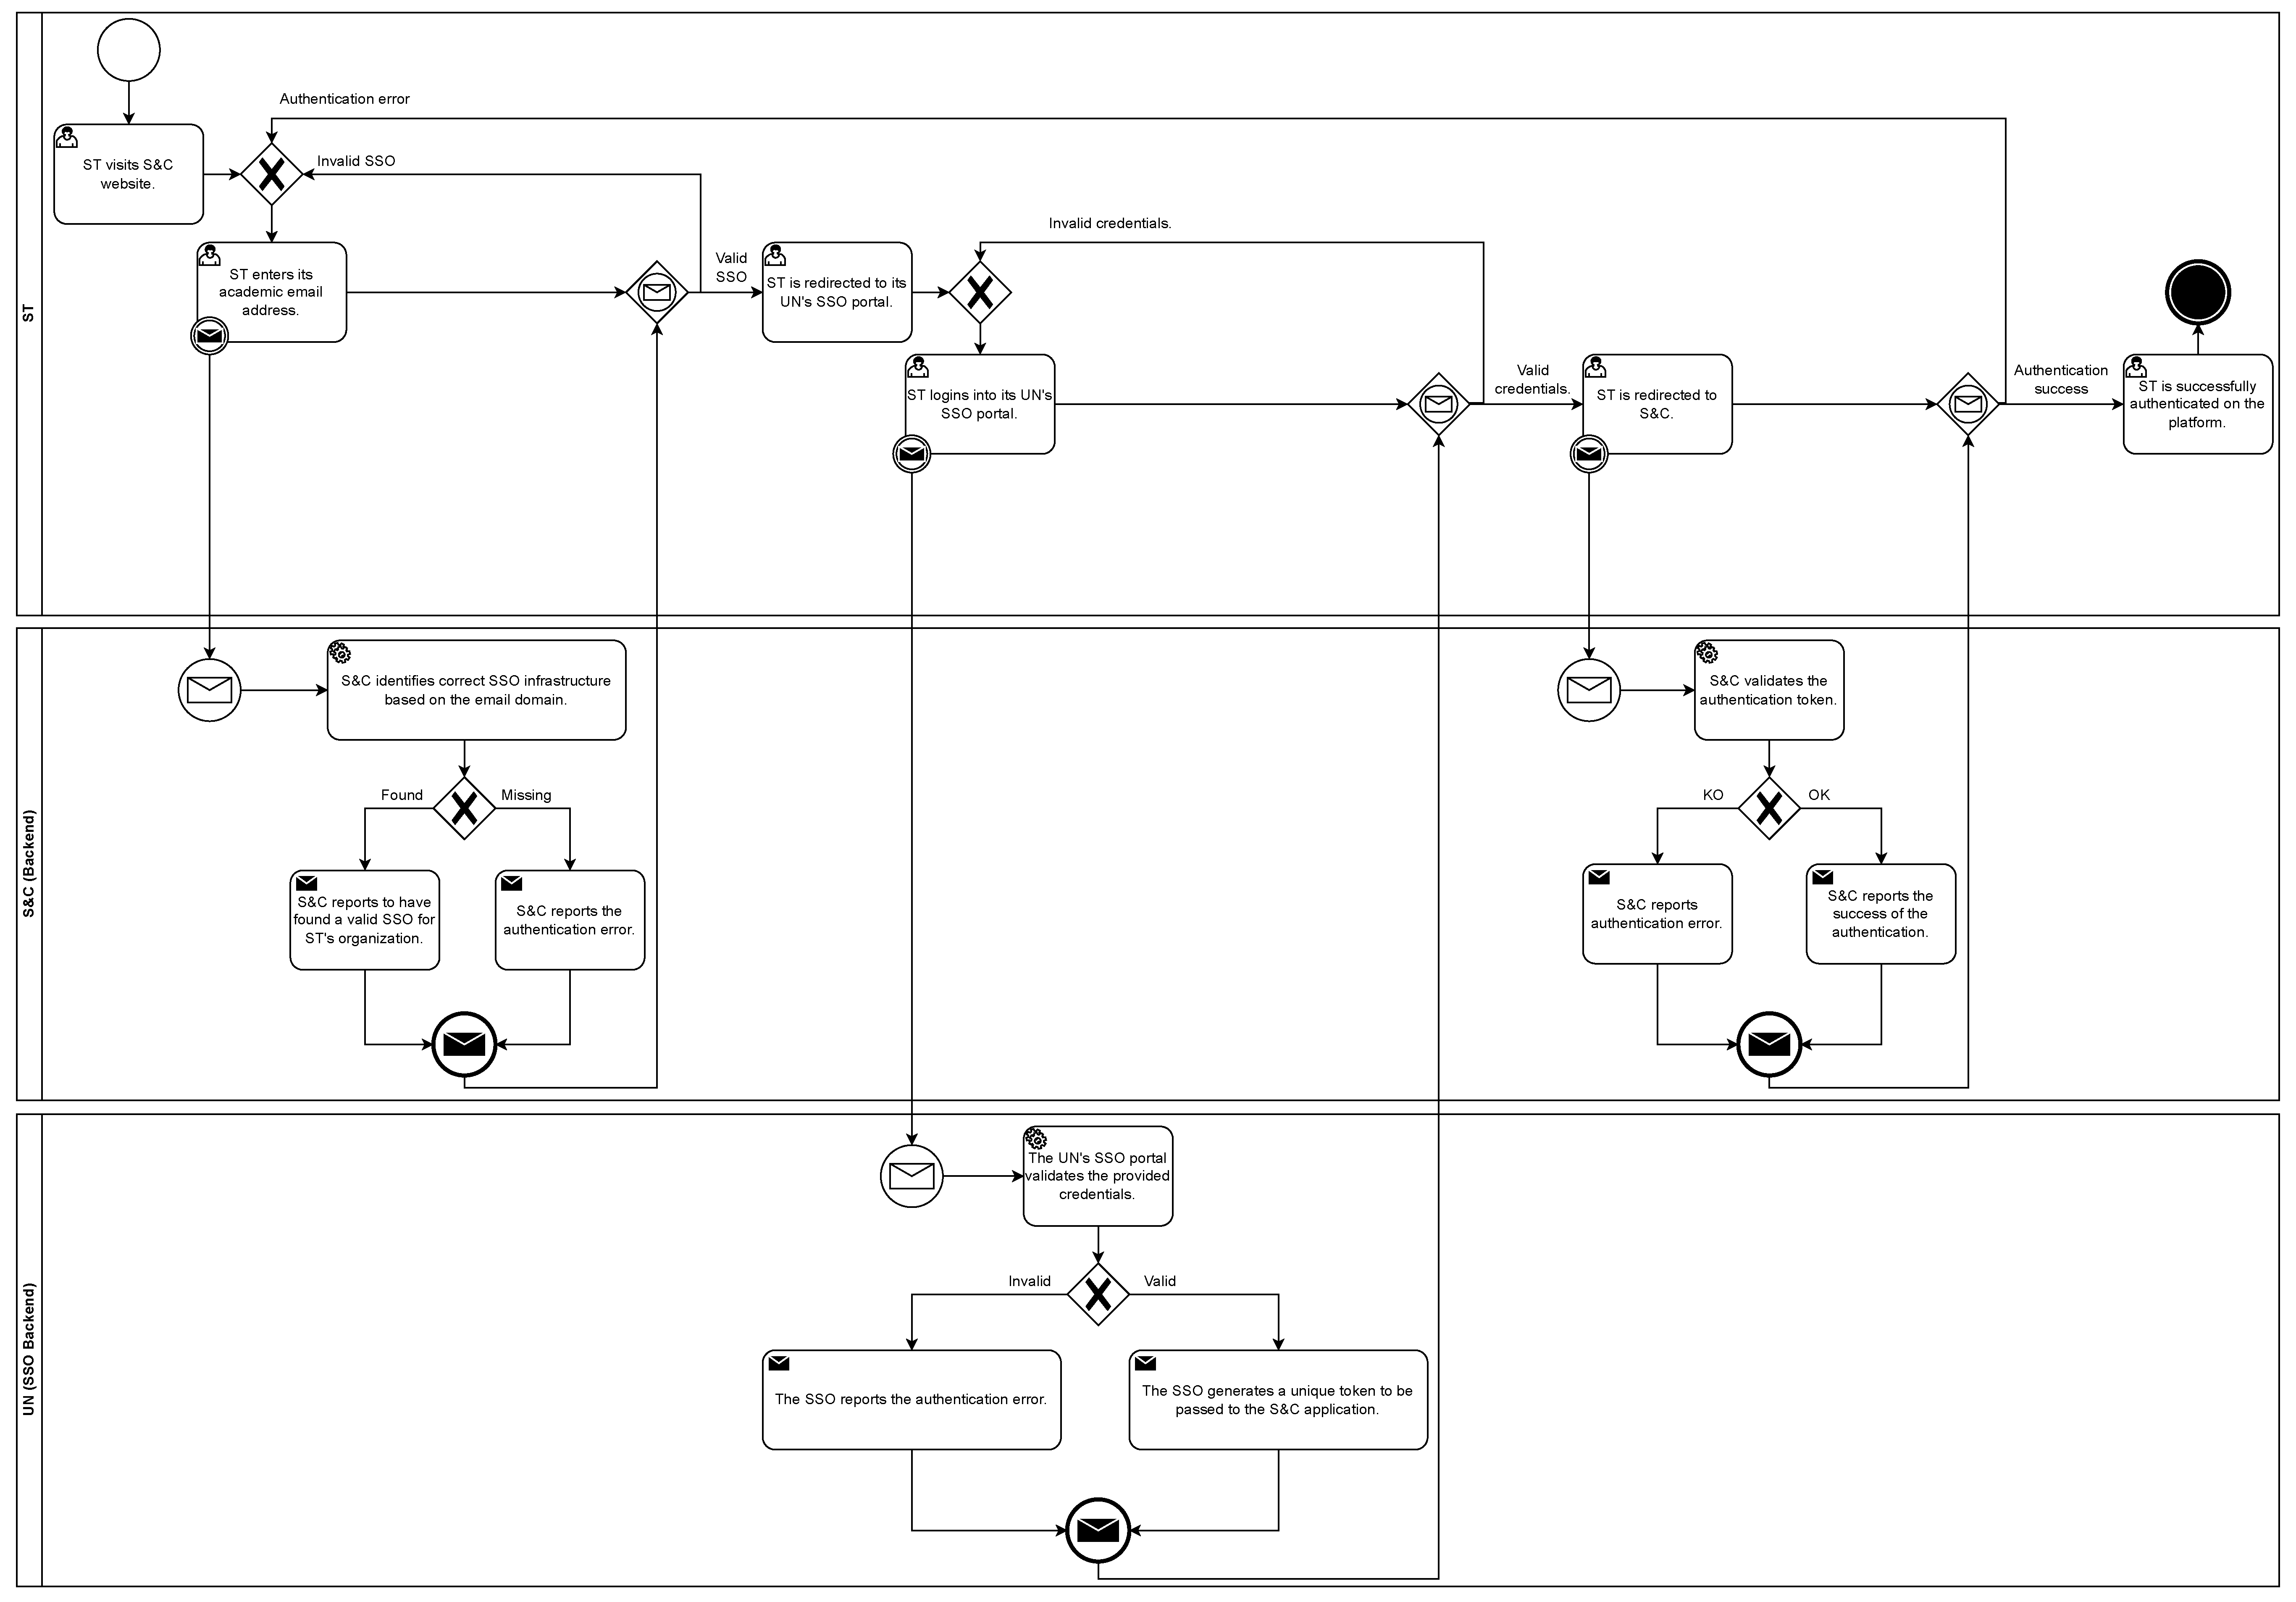
\includegraphics[width=1.0\textwidth]{Images/BPMN_1A.pdf}
                  \caption{ST Enrollment Diagram}
                  \label{fig:st_enrollment_diagram}
            \end{figure}

            % F. 2
      \item \textbf{Account improvements suggestions}:
            S\&C offers an improvement guide by providing to both students and companies ideas on how to improve their
            profile / the internships offers to make them more appealing.

            \begin{figure}[H]
                  \centering
                  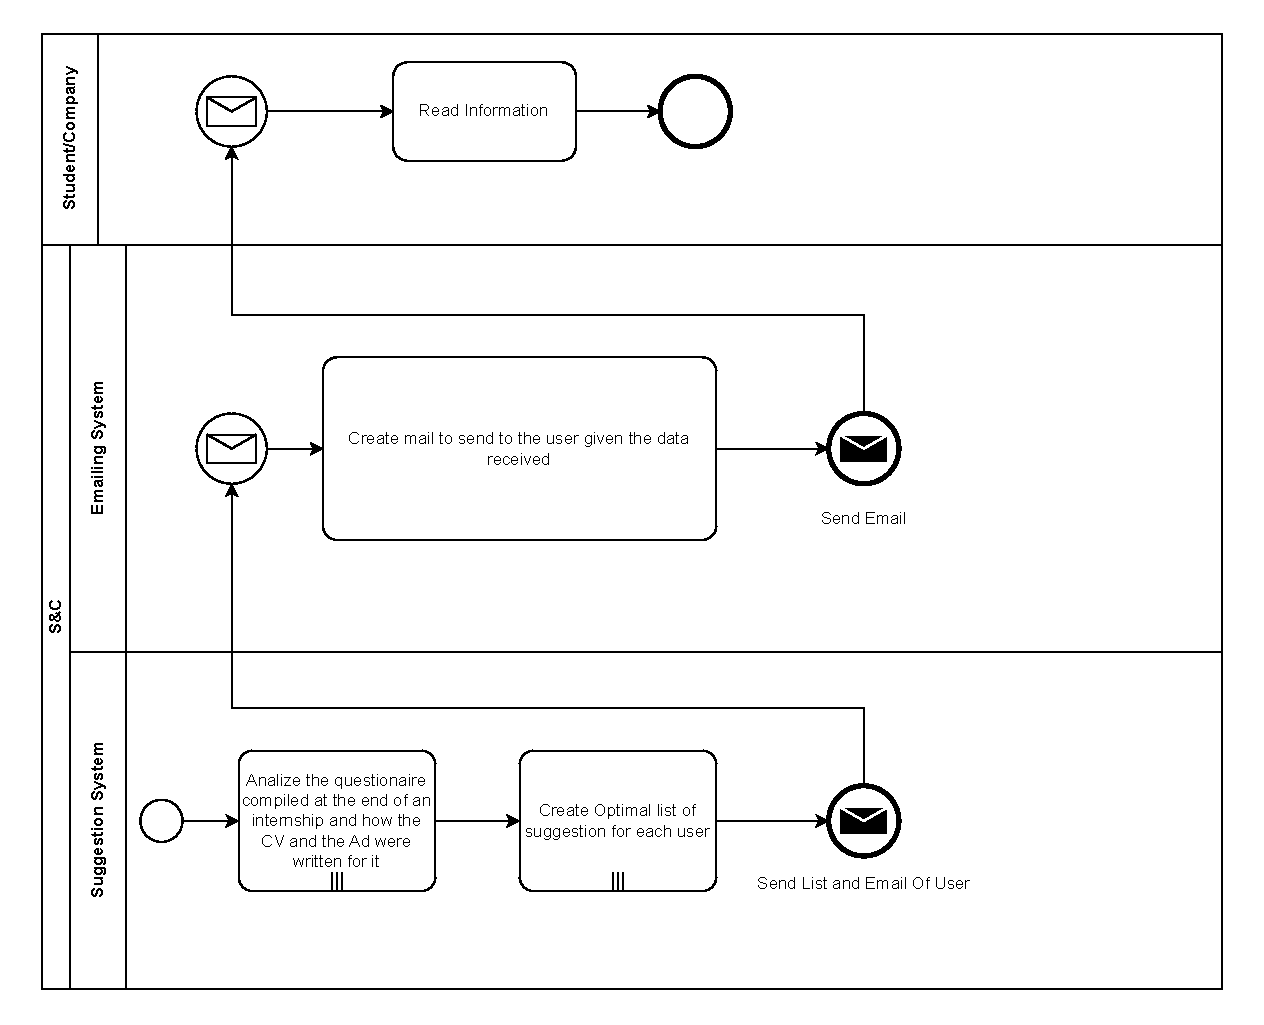
\includegraphics[width=1.0\textwidth]{Images/BPMN_2.pdf}
                  \caption{Account Improvements Suggestions Diagram}
                  \label{fig:account_improvements_suggestions_diagram}
            \end{figure}
\end{itemize}

\par\textbf{Student POV Functionalities}

\begin{itemize}
      % F. 3
      \item \textbf{Edit personal data and add extra information}: This includes the possibility to upload/modify the
            CV at any time.

            \begin{figure}[H]
                  \centering
                  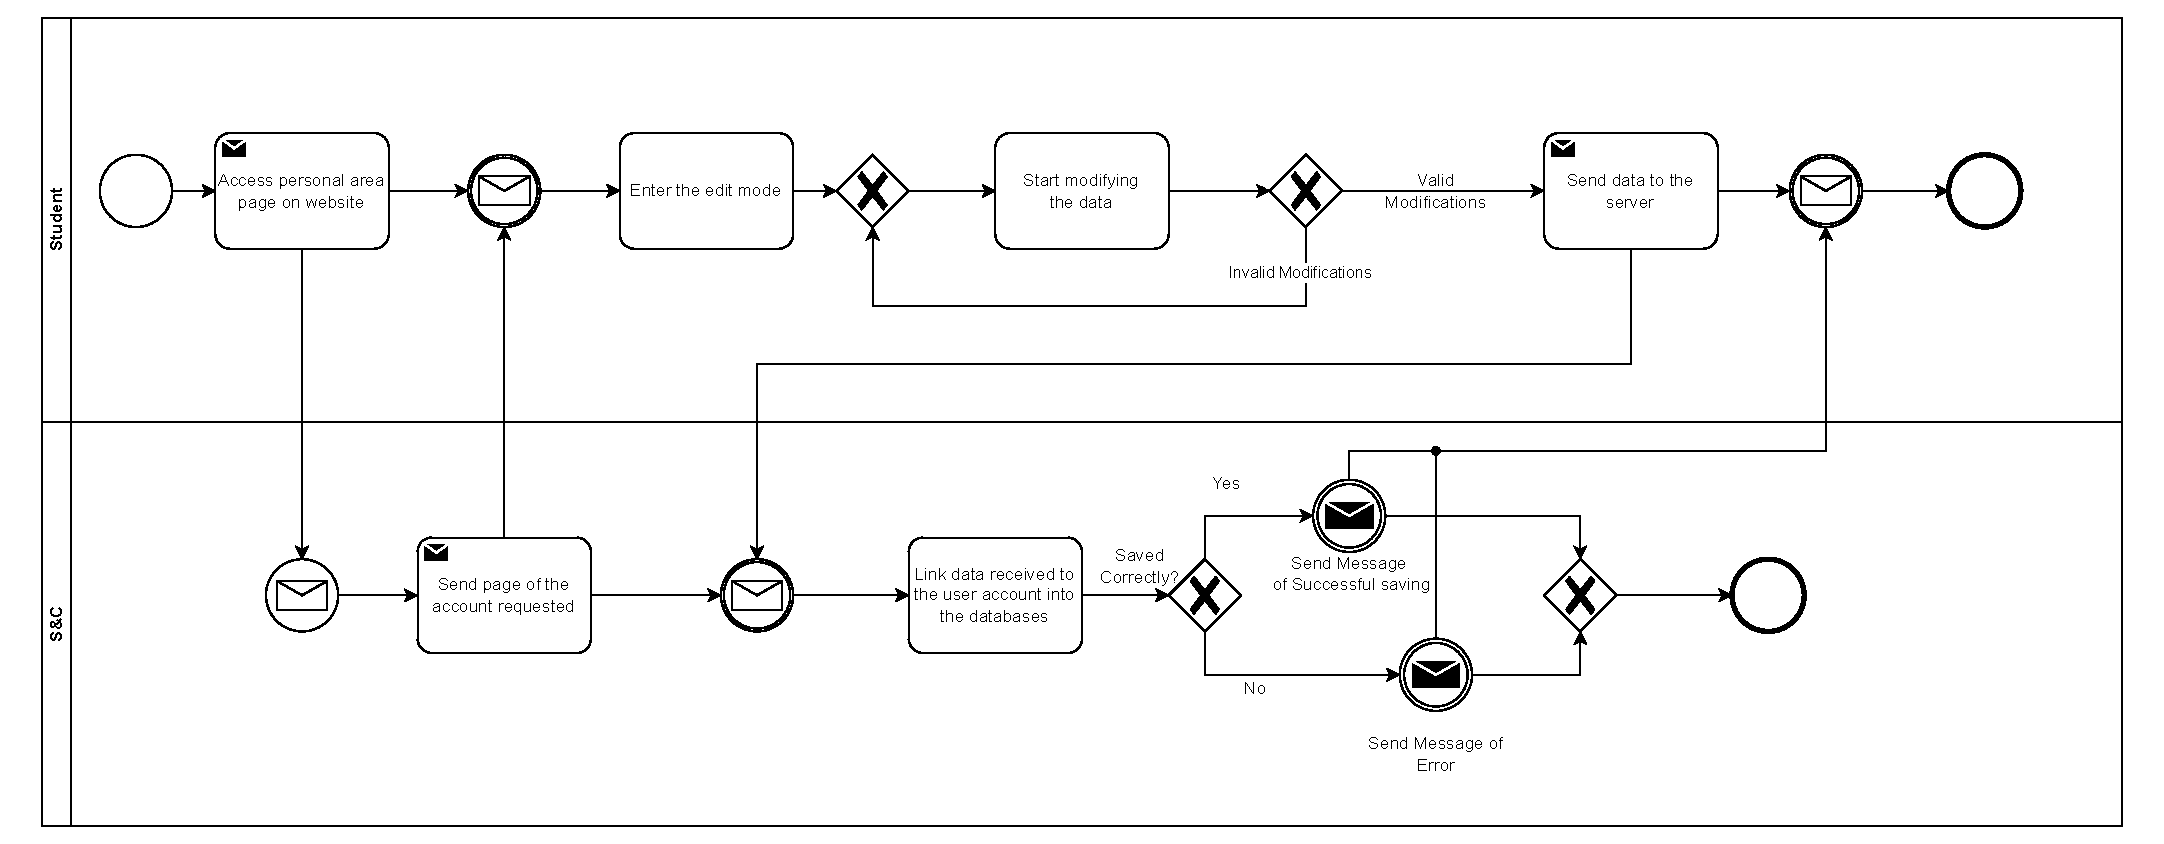
\includegraphics[width=1.0\textwidth]{Images/BPMN_3.pdf}
                  \caption{Edit Personal Data Diagram}
                  \label{fig:edit_personal_data_diagram}
            \end{figure}

            % F. 4
      \item \textbf{Search and apply for internship on the app}: This can be conducted by simple keyword search, but
            there are also more advanced search functionalities to better refine the results. This includes advanced
            search filters, and suggestions based on recent searches. Applying for an internship will also activate
            notifications to the user whenever the application gets accepted/rejected and whenever the questionnaire
            (see next point) from the company is available.

            \begin{figure}[H]
                  \centering
                  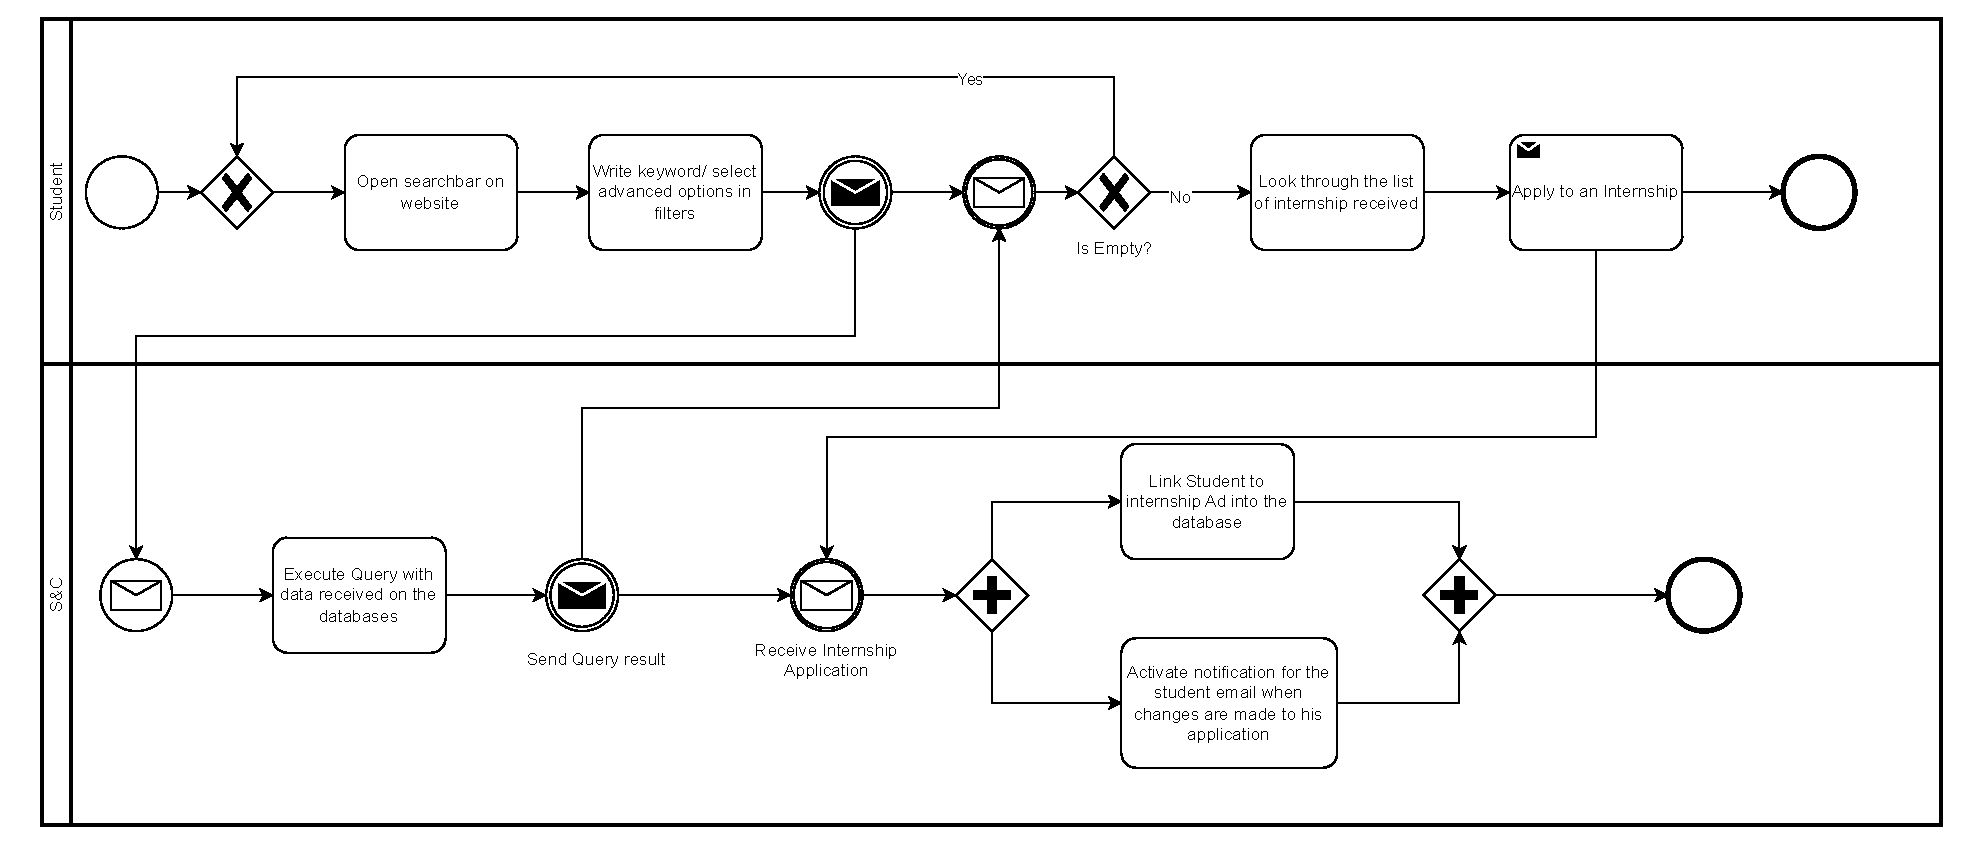
\includegraphics[width=1.0\textwidth]{Images/BPMN_4.pdf}
                  \caption{Search and Apply for Internship Diagram}
                  \label{fig:search_and_apply_for_internship_diagram}
            \end{figure}

            % F. 5
      \item \textbf{Compilation of the questionnaire}: The process of selecting students for an internship is carried
            out through questionnaires. S\&C allows students to compile such questionnaire inside the app and maintain
            partial answers between sessions. Whenever the company has gathered all the results and published them a
            notification will alert the user.

            \begin{figure}[H]
                  \centering
                  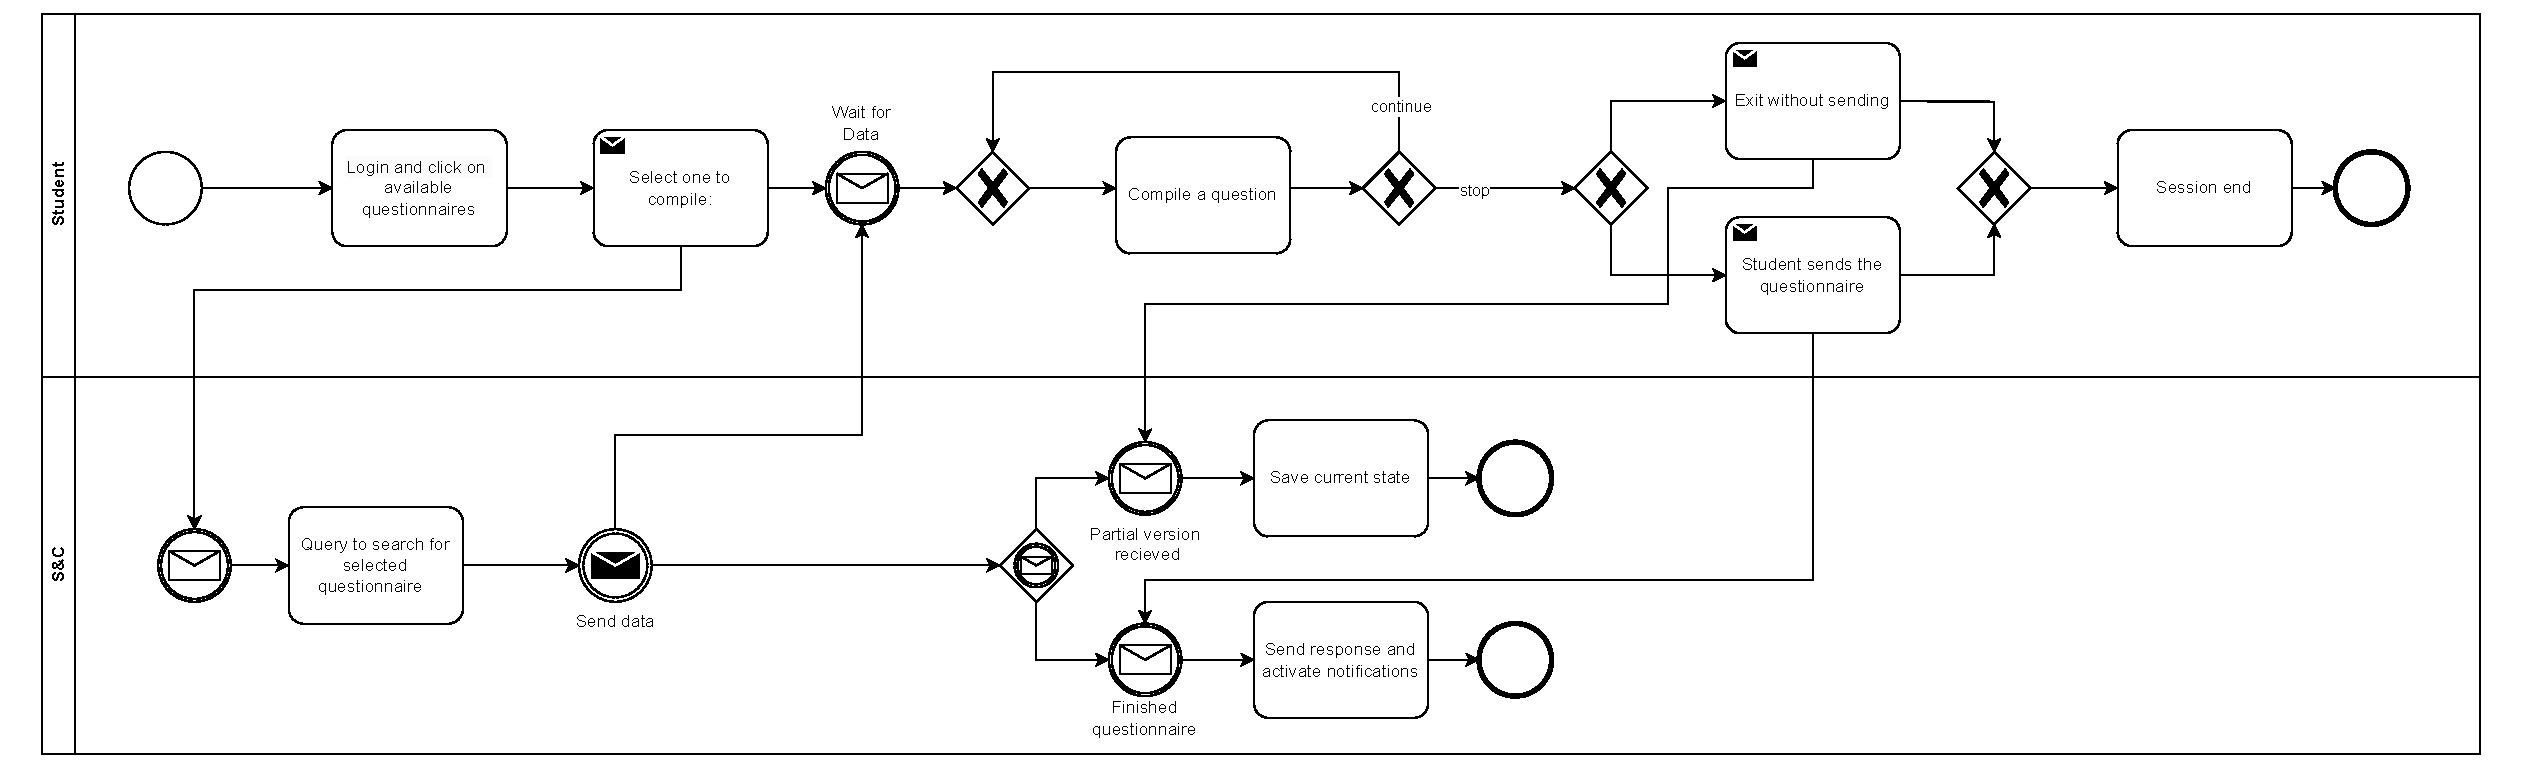
\includegraphics[width=1.0\textwidth]{Images/BPMN_5.pdf}
                  \caption{Compilation of Questionnaire Diagram}
                  \label{fig:compilation_of_the_questionnaire_diagram}
            \end{figure}
            % F. 6
      \item \textbf{Profiling/Recommendation}: This is an advanced functionality that allows students to run an
            algorithm on their personal data and extract structured data regarding their user profile. This data allows
            S\&C to find internships that might interest the student with a Data Driven approach. Student will also get
            notifications from S\&C whenever a new internship that might interest the student gets published.

            \begin{figure}[H]
                  \centering
                  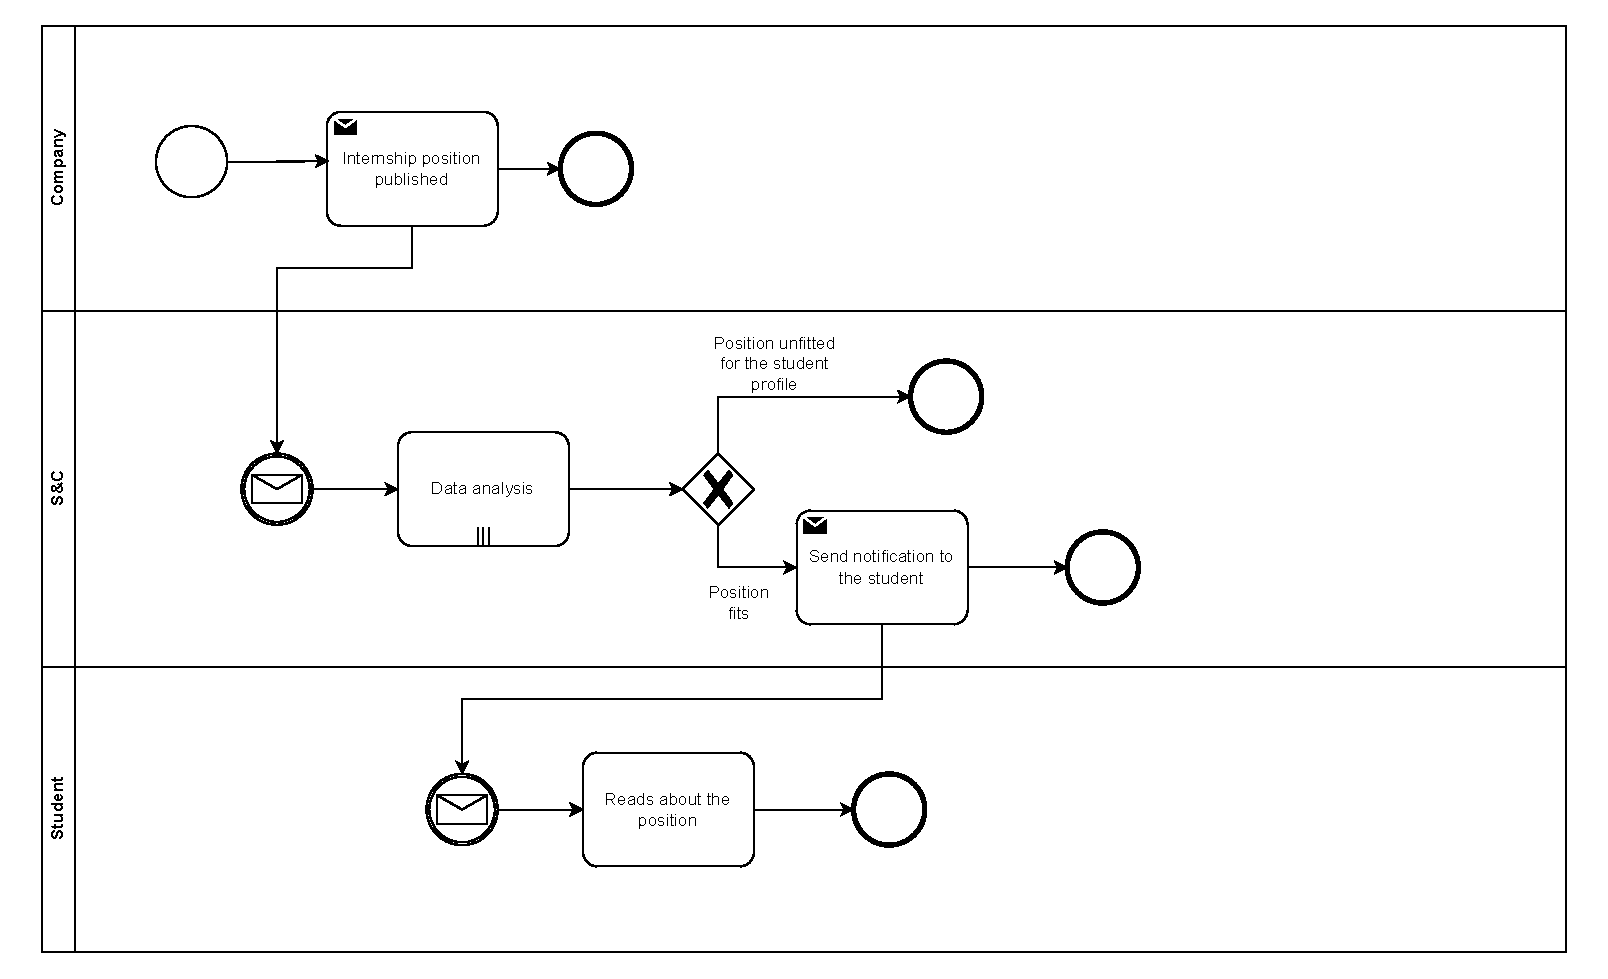
\includegraphics[width=1.0\textwidth]{Images/BPMN_6.pdf}
                  \caption{Profiling/Recommendation Diagram}
                  \label{fig:profiling_recommendation_diagram}
            \end{figure}

\end{itemize}

\par\textbf{Company POV Functionalities}

\begin{itemize}
      % F. 8
      \item \textbf{Edit the company profile}: The company can edit the profile by adding extra descriptive data. The
            aim of this is to allow students to decide where to apply based on the available data. This data also
            supports the suggestion mechanism of S\&C.

            \begin{figure}[H]
                  \centering
                  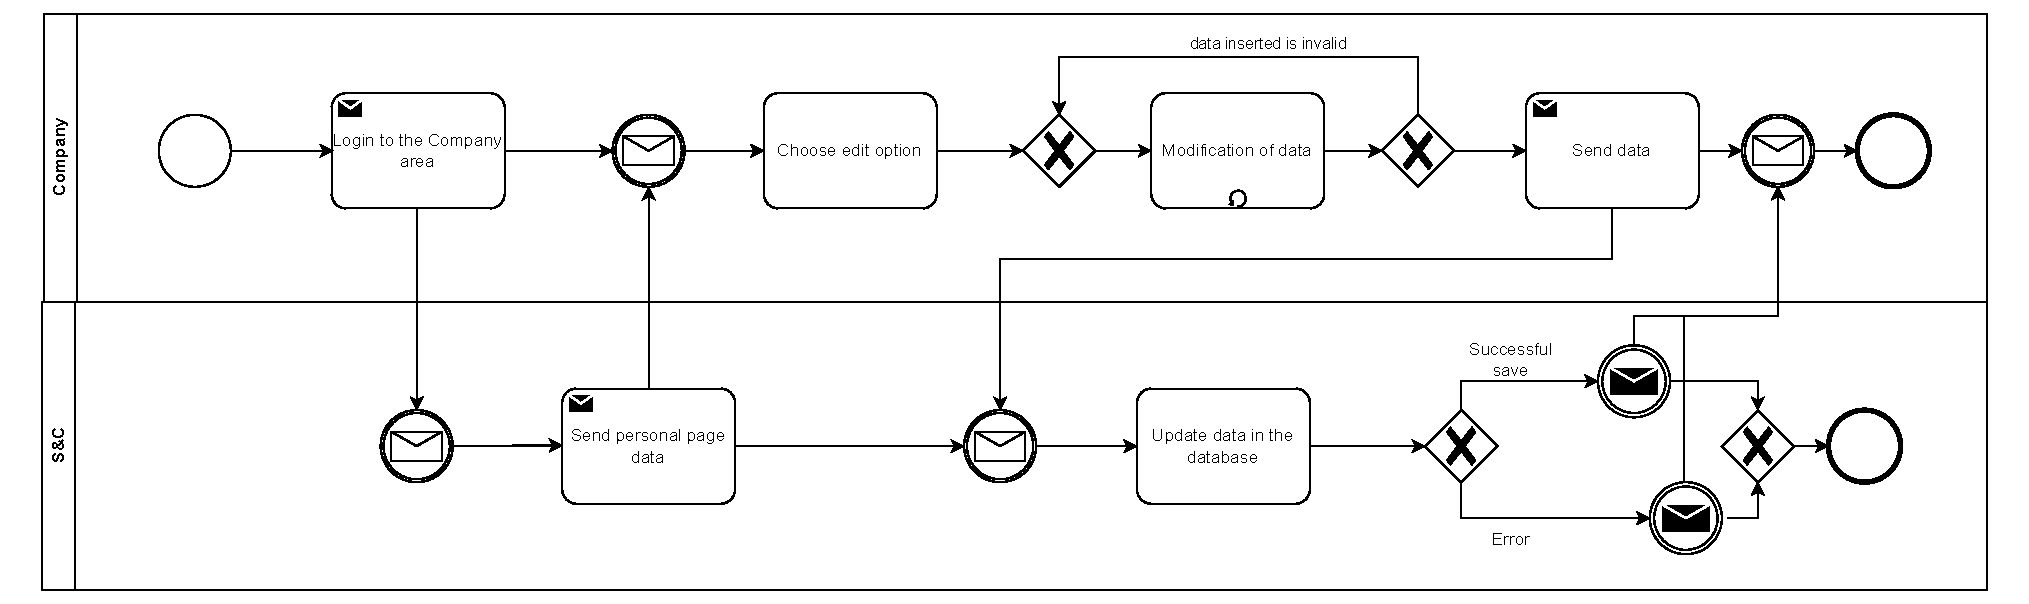
\includegraphics[width=1.0\textwidth]{Images/BPMN_8.pdf}
                  \caption{Edit the Company Profile Diagram}
                  \label{fig:edit_the_company_profile_diagram}
            \end{figure}

            % F. 9
      \item \textbf{Open an internship position}: The main feature of S\&C is the possibility for the company to
            publish information about open positions and advertise them. Interested students are free to apply to them.
            To publish a position the company needs to provide a comprehensive description of the position to guide
            decisions. This is referred to students but also the recommendation system that will try to match
            internships with students. The company also needs to specify a deadline for applications.

            \begin{figure}[H]
                  \centering
                  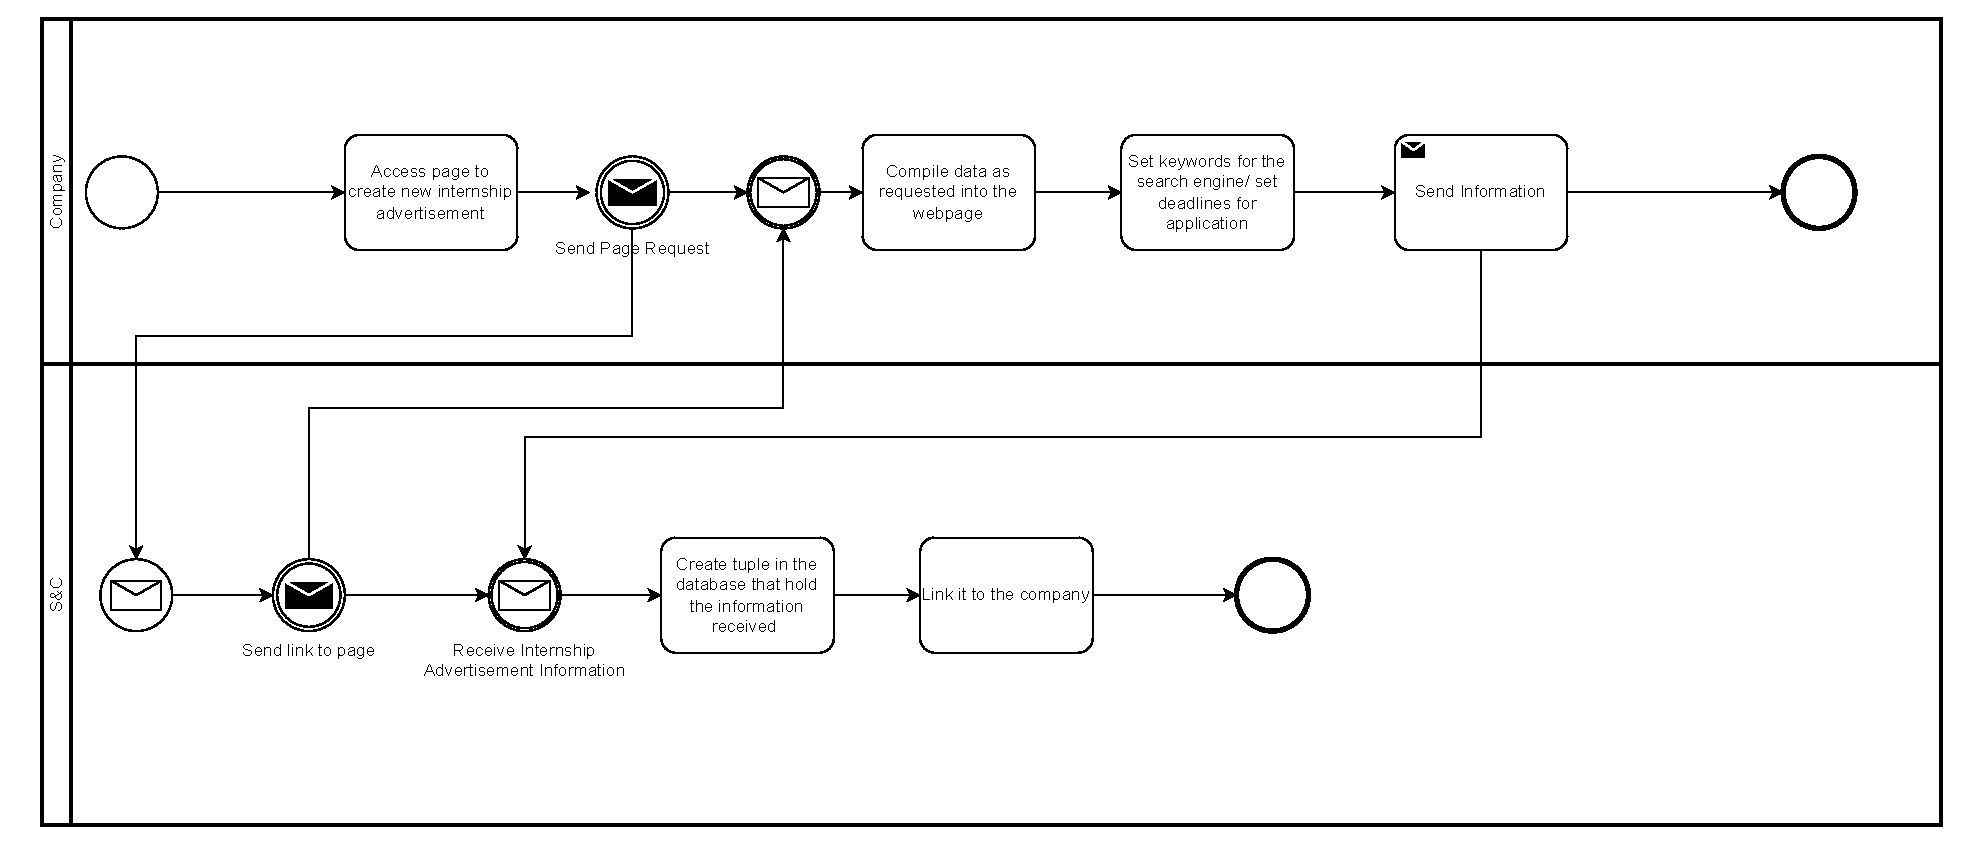
\includegraphics[width=1.0\textwidth]{Images/BPMN_9.pdf}
                  \caption{Open an Internship Position Diagram}
                  \label{fig:open_an_internship_position_diagram}
            \end{figure}

            % F. 10
      \item \textbf{Search suitable students}: The recommendation system previously described in the student section
            works also for companies but with some differences. For privacy reasons companies will see the matched
            students data in an anonymous way. With this feature, companies can invite suitable students to take part
            in the selection process. To gain access to more information about the student, including contact
            information, the selection process must go through, this means the student must take the questionnaire and
            get selected.

            \begin{figure}[H]
                  \centering
                  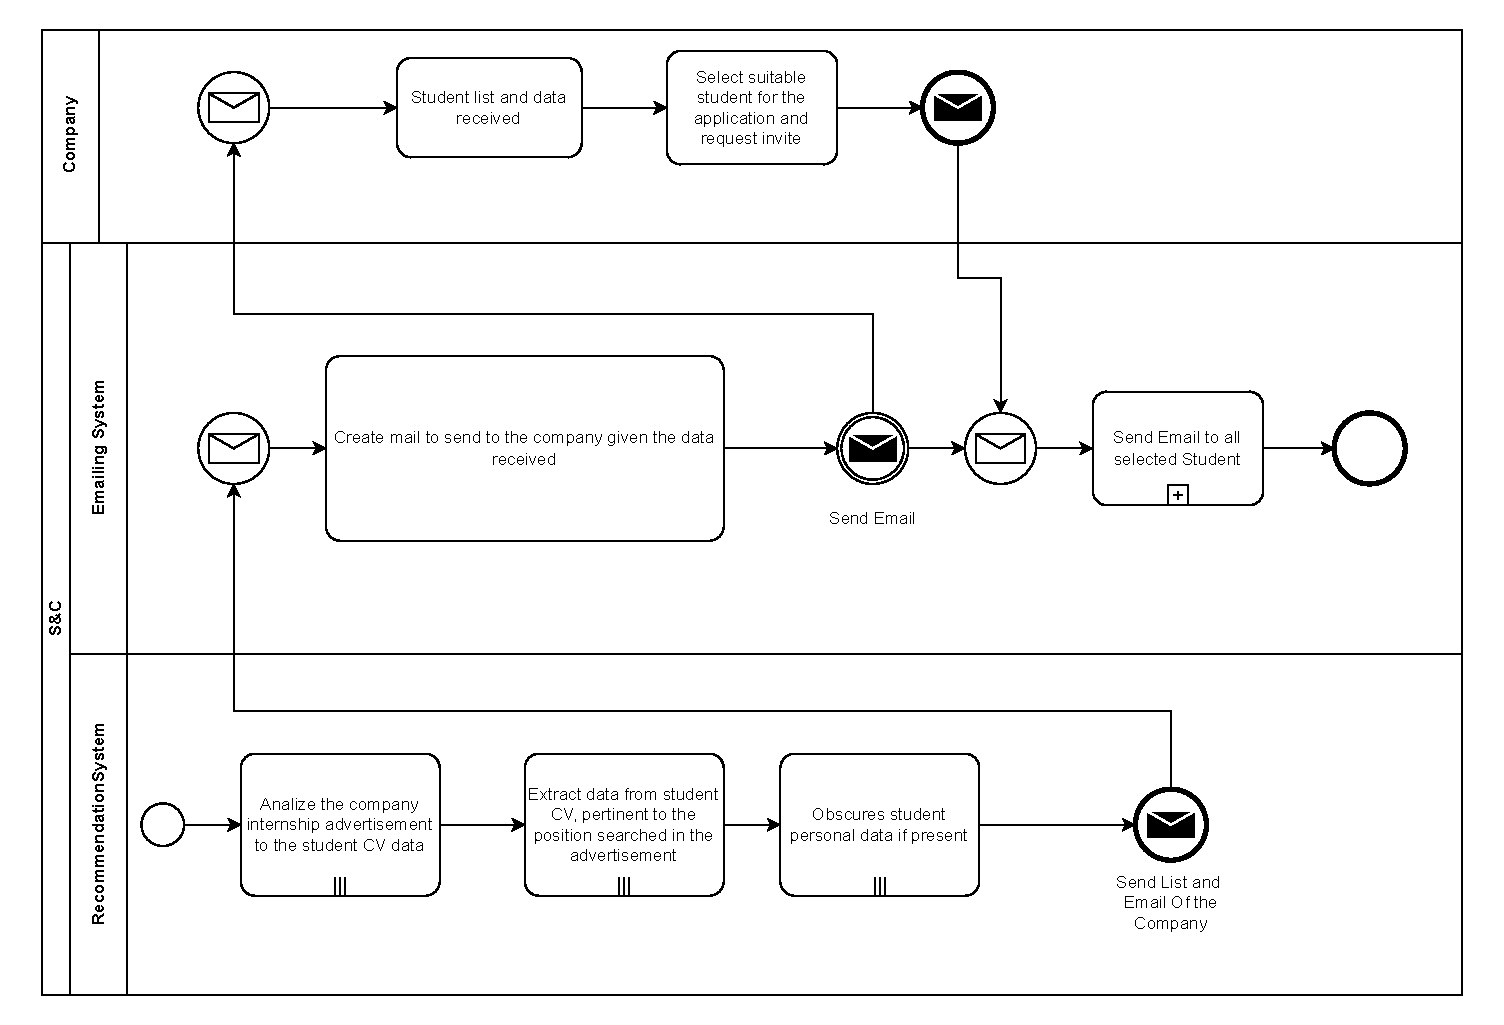
\includegraphics[width=1.0\textwidth]{Images/BPMN_10.pdf}
                  \caption{Search Suitable Students Diagram}
                  \label{fig:search_suitable_students_diagram}
            \end{figure}

            % F. 11
      \item \textbf{Create and post personalized questionnaires for the selection phase}: S\&C allows creating and
            customizing questionnaires inside the application to later give them to students as part of the selection
            process. The S\&C application also gathers the answers provided by the students and allows viewing them in
            a structured manner so that the company can easily filter/sort/analyze them and choose the candidates.

            \begin{figure}[H]
                  \centering
                  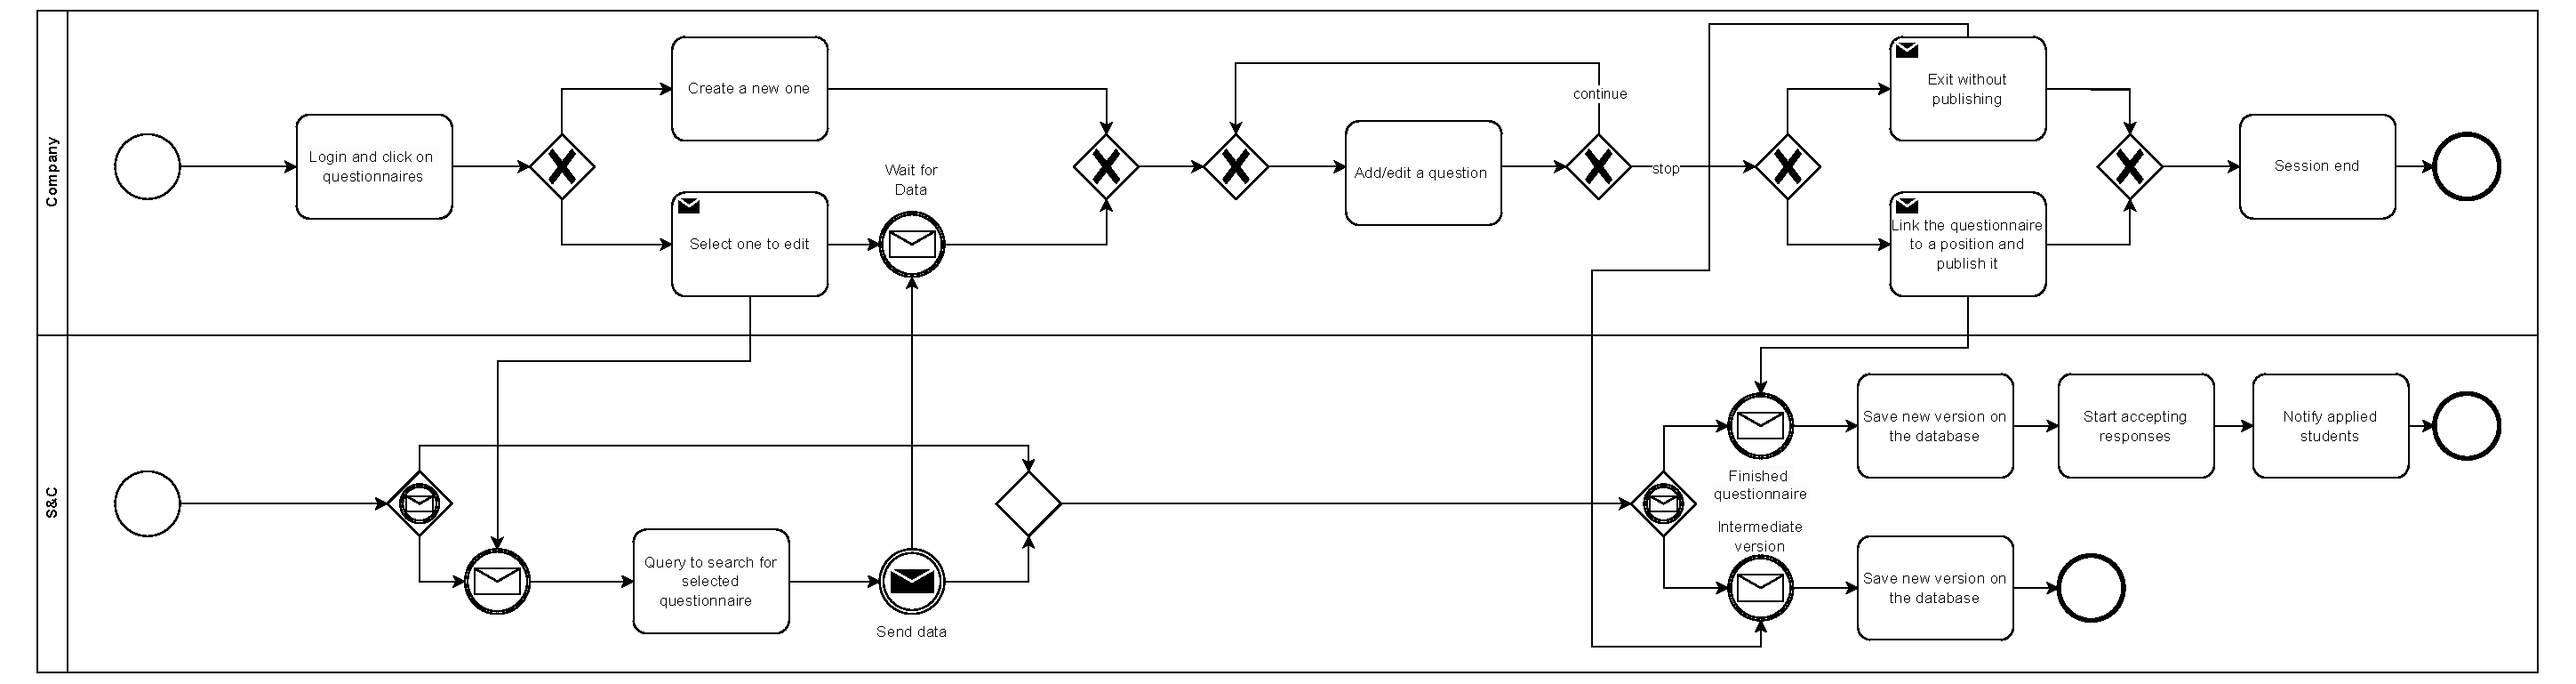
\includegraphics[width=1.0\textwidth]{Images/BPMN_11.pdf}
                  \caption{Create and Post Personalized Questionnaires for the Selection Phase Diagram}
                  \label{fig:create_and_post_personalized_questionnaires_for_the_selection_phase_diagram}
            \end{figure}

            % F. 13
      \item \textbf{Monitoring}: This functionality is used by the company to keep track of all the internships
            currently active and monitor how they are going (e.g., if there were complaints, etc.), but also see all
            the past internships for historical data.

            \begin{figure}[H]
                  \centering
                  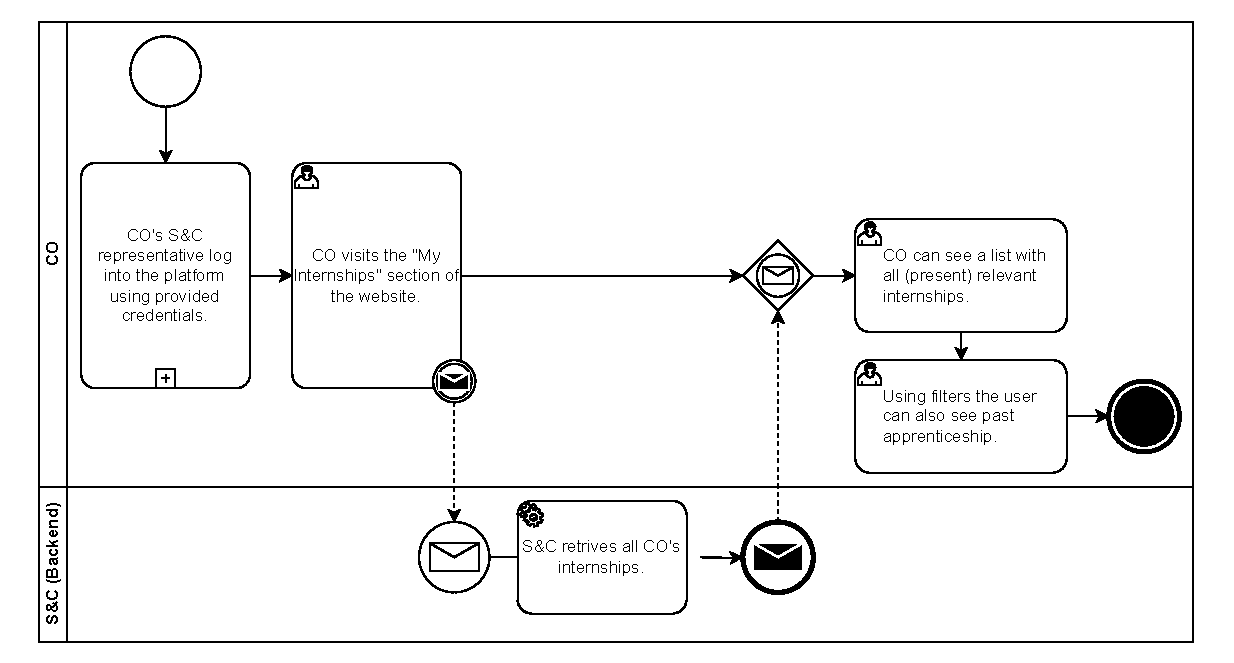
\includegraphics[width=1.0\textwidth]{Images/BPMN_13.pdf}
                  \caption{CO Monitoring Diagram}
                  \label{fig:co_monitoring_diagram}
            \end{figure}

\end{itemize}

\par\textbf{University POV Functionalities}

\begin{itemize}
      % F. 14
      \item \textbf{Monitoring}: S\&C keeps track of all the interactions between students and companies (applications
            and internships). The universities can access the portion of this data regarding their own students for
            analysis.

            \begin{figure}[H]
                  \centering
                  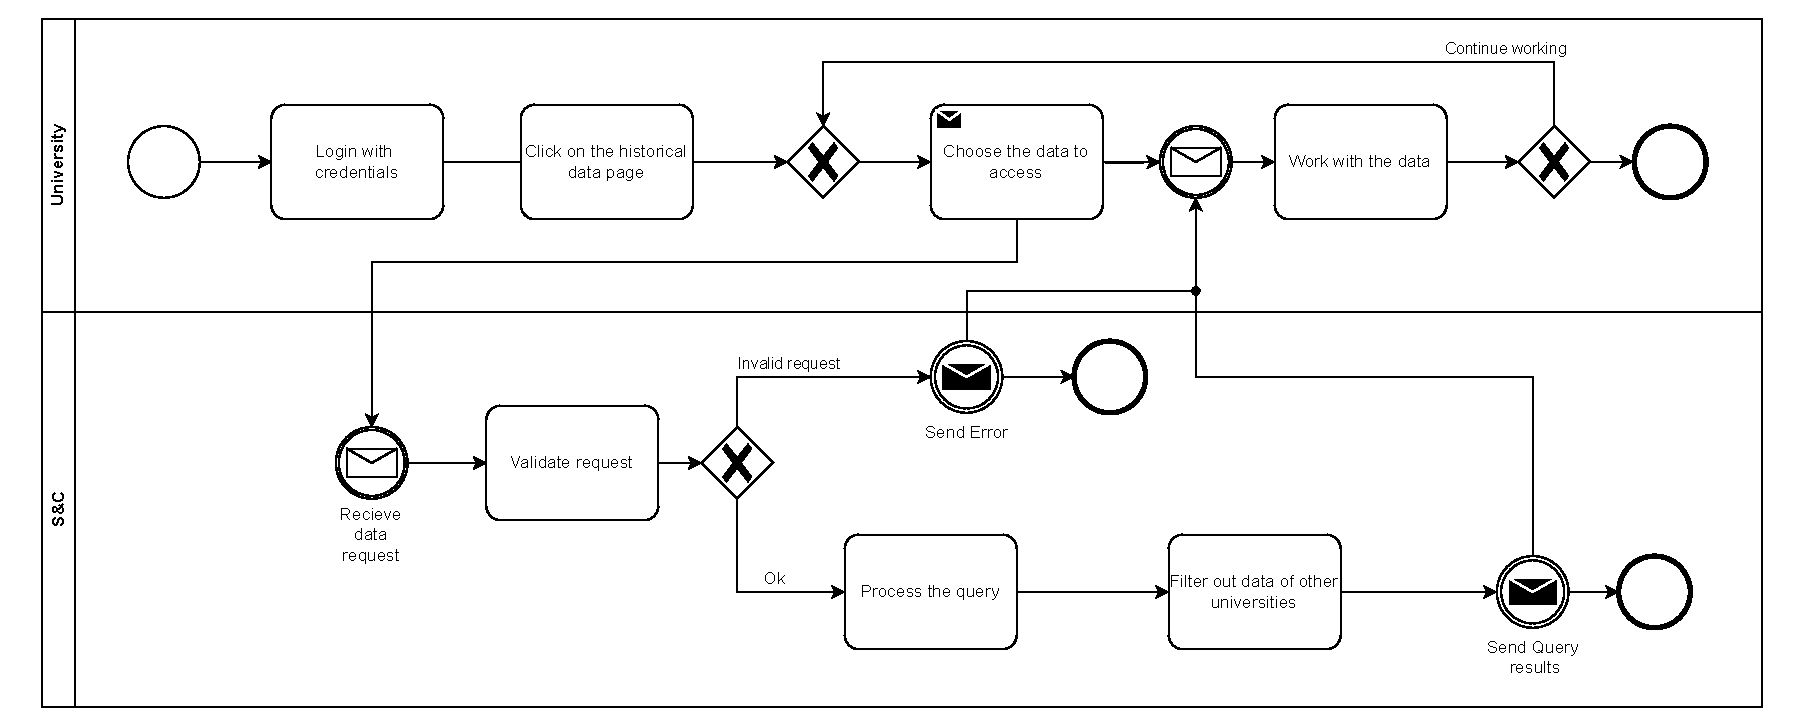
\includegraphics[width=1.0\textwidth]{Images/BPMN_14.pdf}
                  \caption{UN Monitoring Diagram}
                  \label{fig:un_monitoring_diagram}
            \end{figure}
            % F. 15
      \item \textbf{Complaint handling}: Universities play an important role in the interaction between students and
            companies during the internship period. If any problem arises during such a period, a student can open a
            complaint ticket. The university steps in to handle the problem by acting as a third party. In the
            worst-case scenario, the suspension or cancellation of the internship is an available option to the
            university.

            \begin{figure}[H]
                  \centering
                  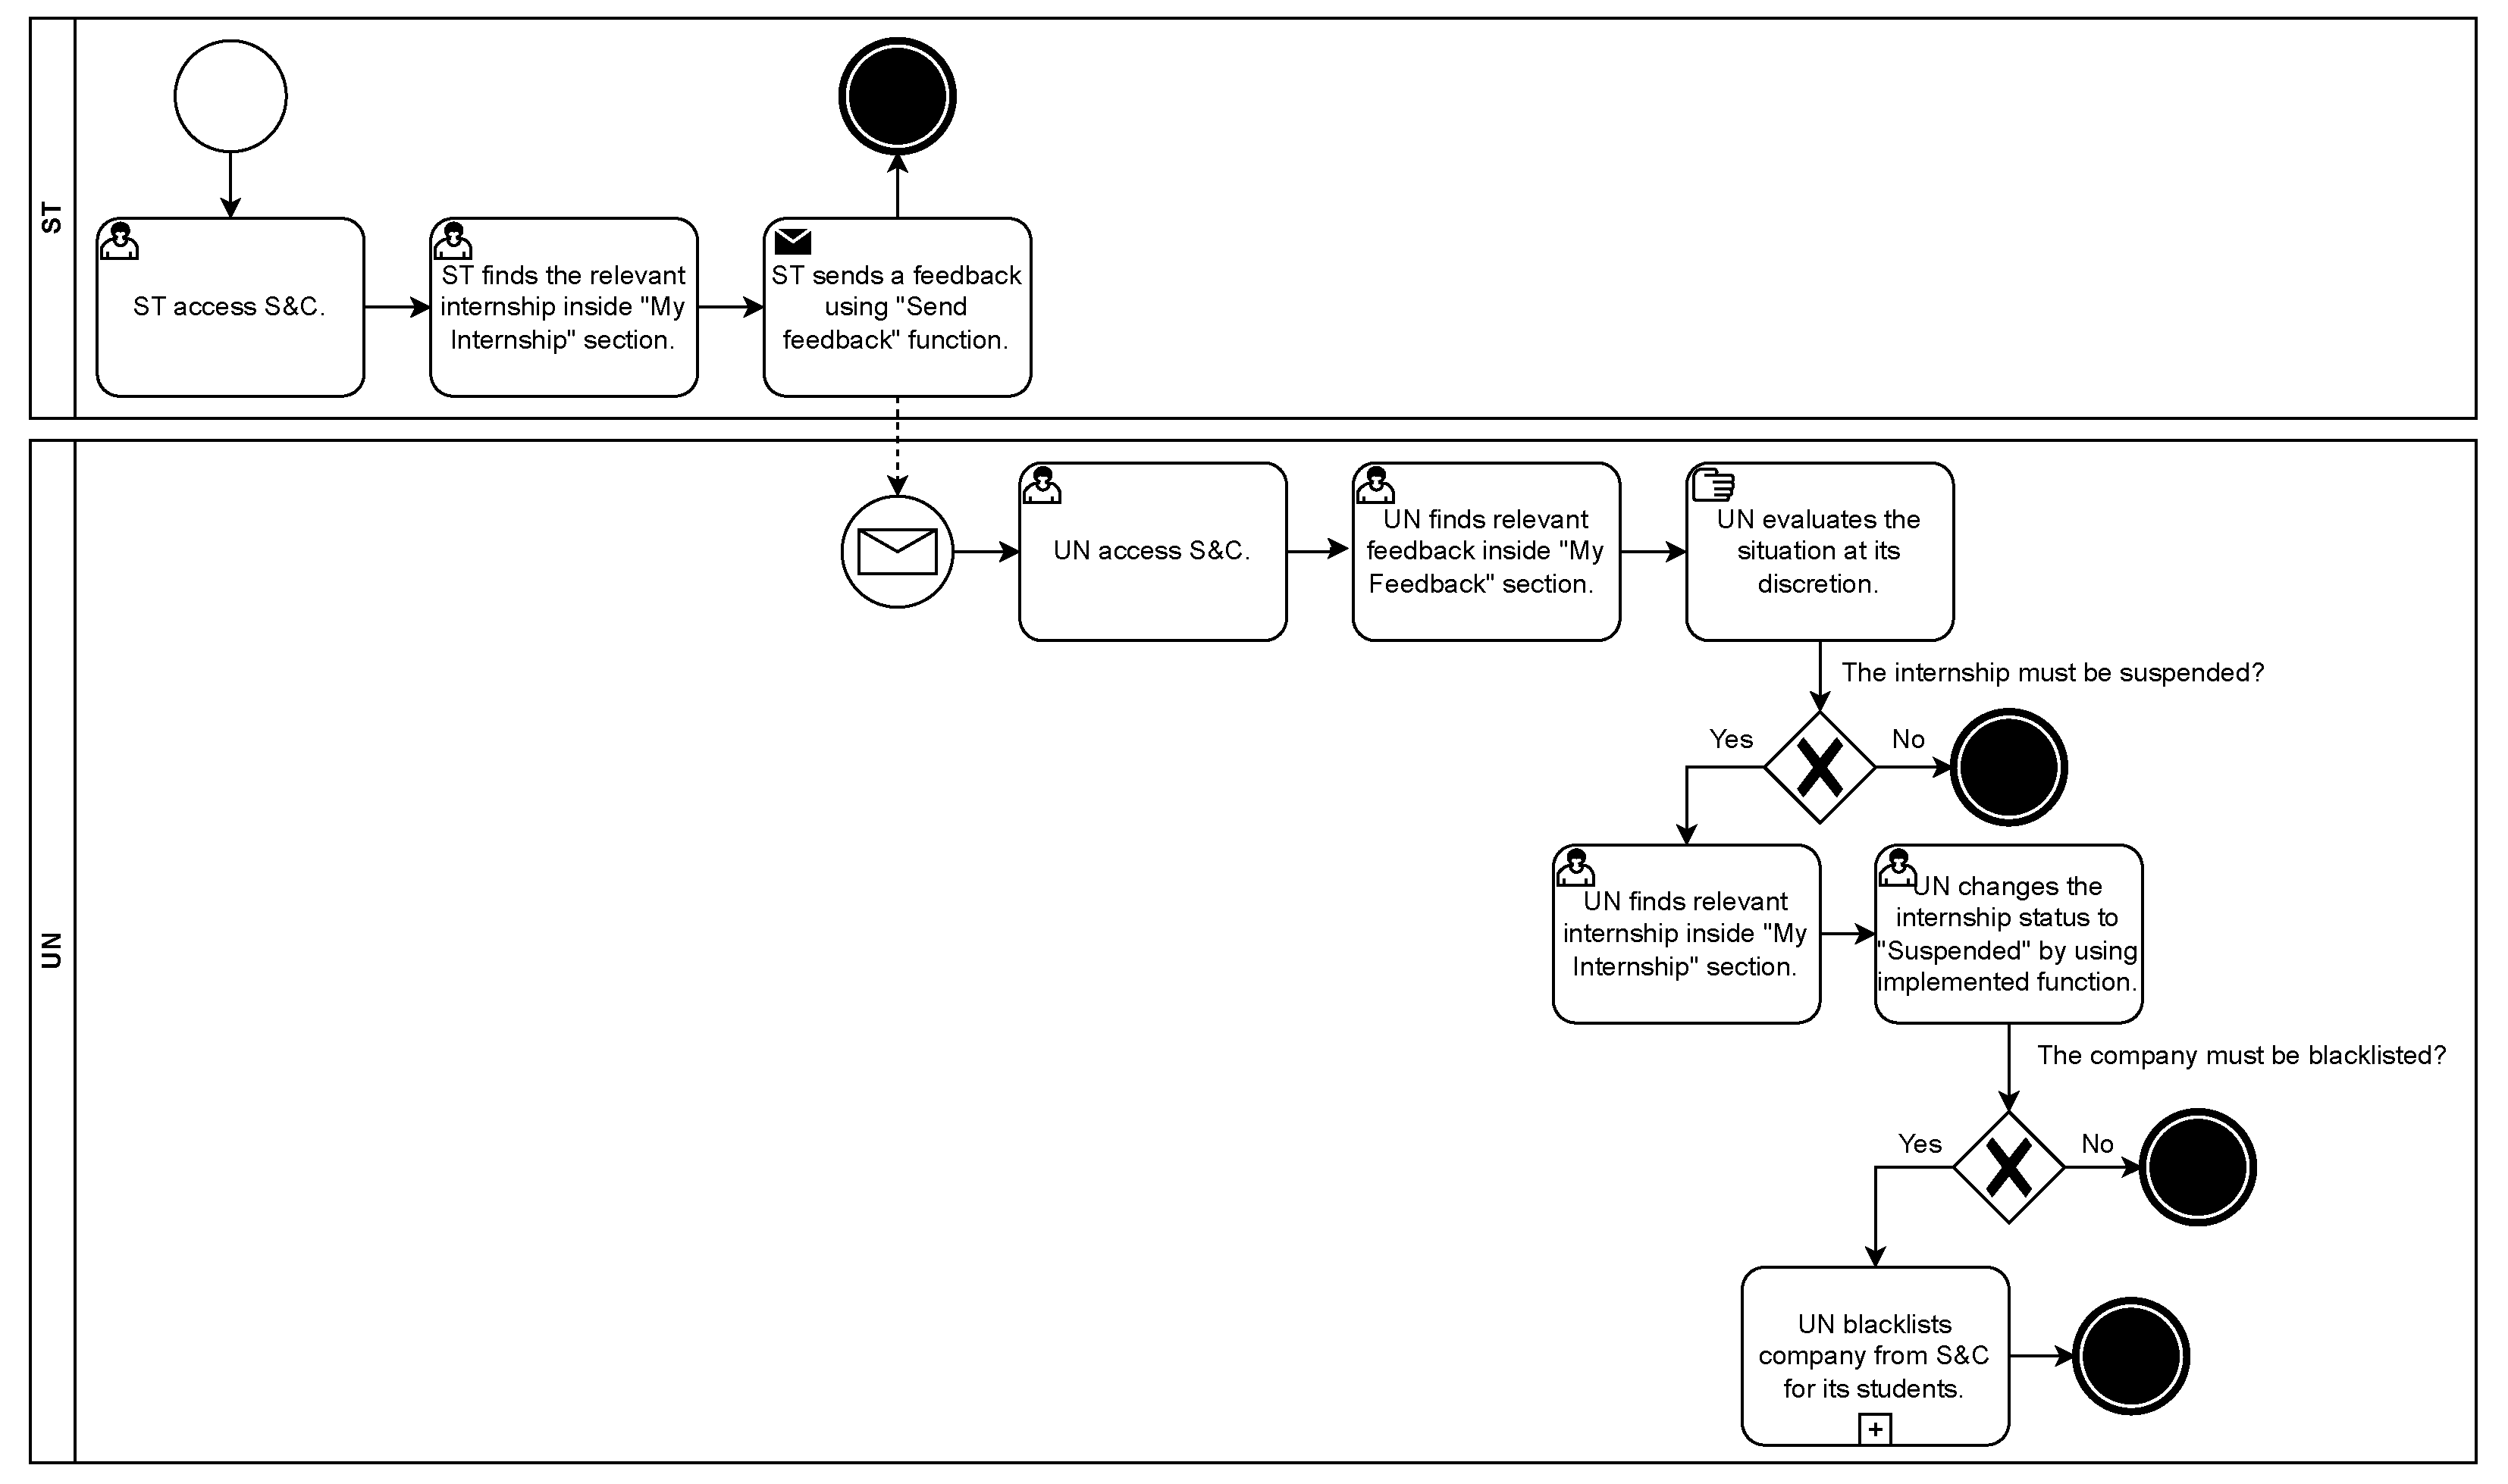
\includegraphics[width=1.0\textwidth]{Images/BPMN_15.pdf}
                  \caption{UN Complaint Handling Diagram}
                  \label{fig:un_complaint_handling_diagram}
            \end{figure}

            % F. 16
      \item \textbf{Blacklisting}: If the university deems a company untrustworthy or has been subject to multiple
            complaints, it can blacklist it. This ensures that students at such university can’t see the company and
            vice versa, the company can’t see the university students.

            \begin{figure}[H]
                  \centering
                  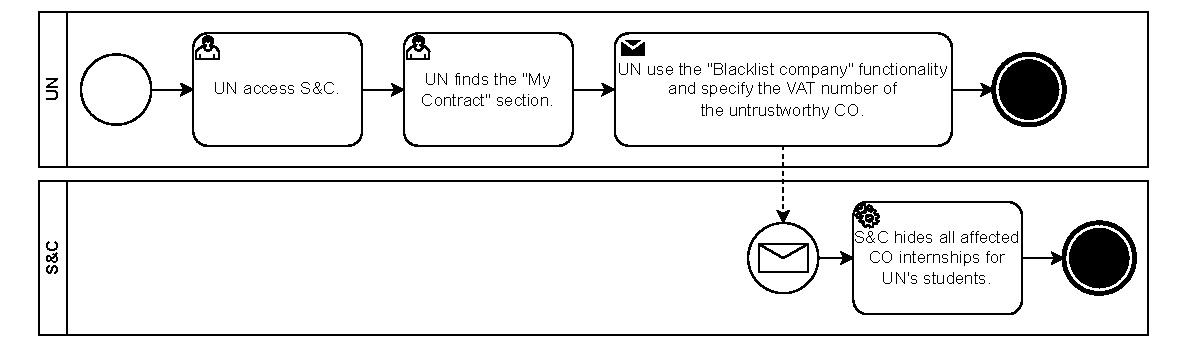
\includegraphics[width=1.0\textwidth]{Images/BPMN_16.pdf}
                  \caption{UN Blacklisting Diagram}
                  \label{fig:un_blacklisting_diagram}
            \end{figure}

\end{itemize}

\section{User Characteristics}
\label{sec:user_characteristics}%

\par The system is designed to be used by three main actors: students, companies, and universities.

\begin{enumerate}
      \item \textbf{Students (STs)}: are verified users who access S\&C through their university credentials to find and
            apply for internships.
            \begin{enumerate}
                  \item They manage their profiles, upload CVs, and participate in company selection processes through
                        questionnaires.
                  \item The platform helps them by suggesting CV improvements and recommending relevant opportunities,
                        while also allowing them to provide feedback on their internship experiences.
            \end{enumerate}
      \item \textbf{Companies (COs)}: join S\&C through formal contracts and use the platform to post internship
            opportunities and recruit students.
            \begin{enumerate}
                  \item They maintain a corporate presence on the platform by creating detailed company profiles that
                        showcase their organization to potential interns.
                  \item They create detailed job listings, evaluate candidates through customized questionnaires, and
                        access anonymized student profiles that match their requirements (and can invite them to apply to
                        their job posting).
                  \item The platform allows them to manage the entire recruitment process, from selection to internship
                        completion, and can provide performance feedback if needed.
            \end{enumerate}
      \item \textbf{Universities (UNs)}: act as overseers of the platform, protecting their students' interests while
            monitoring internship activities.
            \begin{enumerate}
                  \item They have the authority to handle complaints, suspend internships, and blacklist problematic
                        companies.
                  \item Through their integration with S\&C, they can track their students' professional experiences and
                        provide secure authentication for student access by leveraging their existing infrastructure.
            \end{enumerate}
\end{enumerate}

\section{Assumptions, Dependencies and Constraints}
\label{sec:assumptions_dependencies_and_constraints}%

\subsection{Assumptions}
\label{sub:assumptions}%

\begin{longtable}{|l|p{0.9\textwidth}|}
      \hline
      \textbf{Assumption} & \textbf{Description}                                                                   \\
      \hline
      A01                 & Universities designate an individual to manage interactions with the website.          \\
      \hline
      A02                 & Companies have a designated HR representative to manage interactions with the website. \\
      \hline
      A03                 & Companies create internship advertisements based on positions that need to be filled.  \\
      \hline
      A04                 & Students create their CVs using standard templates to facilitate analysis.             \\
      \hline

      \caption{Domain Assumptions}
      \label{tab:domain_assumptions}
\end{longtable}

\subsection{Dependencies}
\label{sub:dependencies}%

\begin{longtable}{|l|p{0.9\textwidth}|}
      \hline
      \textbf{Dependency} & \textbf{Description}                                                          \\
      \hline
      D01                 & The website requires the University's Single Sign-On (SSO) for secure access. \\
      \hline
      D02                 & S\&C needs to communicate correctly with the emailing system.                 \\
      \hline

      \caption{Domain Dependencies}
      \label{tab:domain_dependencies}
\end{longtable}

\subsection{Constraints}
\label{sub:constraints}%

\begin{longtable}{|l|p{0.9\textwidth}|}
      \hline
      \textbf{Constraint} & \textbf{Description}                                            \\
      \hline
      C01                 & All users must have the adequate devices to access the website. \\
      \hline

      \caption{Domain Constraints}
      \label{tab:domain_constraints}
\end{longtable}
